%=====================================================================
% Reporte tecnico v2: Propuesta extendida del modelo vectorial ReNoN-Azuay
% con metodos en la frontera del conocimiento (autoencoders, KAN,
% atencion, Dream Optimization Algorithm) y simulaciones en MATLAB.
% Proyecto: Transicion energetica sostenible en Azuay-Ecuador (XXII Concurso VIUC)
% DEET - Universidad de Cuenca
%=====================================================================
\documentclass[11pt,a4paper]{article}
\usepackage[utf8]{inputenc}
\usepackage[T1]{fontenc}
\usepackage[spanish,es-tabla]{babel}
\usepackage[top=2.6cm,bottom=2.6cm,left=2.8cm,right=2.4cm]{geometry}
\usepackage{graphicx}
\usepackage[table]{xcolor}
\usepackage{booktabs}
\usepackage{amsmath,amssymb,bm}
\usepackage{caption}
\usepackage{siunitx}
\sisetup{output-decimal-marker={,},group-separator={\,}}
\usepackage{enumitem}
\usepackage{fancyhdr}
\usepackage{multirow}
\usepackage{longtable}
\usepackage{array}
\newcolumntype{L}[1]{>{\raggedright\arraybackslash}p{#1}}
\usepackage{url}
\usepackage{textcomp}
\usepackage[hidelinks]{hyperref}

\definecolor{UCblue}{RGB}{0,40,86}
\definecolor{UCred}{RGB}{165,16,8}
\definecolor{UCbluelight}{RGB}{230,236,244}
\captionsetup{font=small,labelfont={bf,color=UCblue}}
\usepackage{sectsty}
\sectionfont{\color{UCblue}}
\subsectionfont{\color{UCblue}}
\subsubsectionfont{\color{UCblue}}

\pagestyle{fancy}
\fancyhf{}
\fancyhead[L]{\small\color{UCblue} Proyecto ReNoN--Azuay · XXII Concurso VIUC · Reporte t\'ecnico v2}
\fancyhead[R]{\small\color{UCblue} DEET -- Universidad de Cuenca}
\fancyfoot[C]{\small\thepage}
\renewcommand{\headrulewidth}{0.4pt}

\newcommand{\vect}[1]{\bm{#1}}
\newcommand{\CO}{CO$_2$}

\title{\color{UCblue}\textbf{Propuesta t\'ecnica extendida: modelo vectorial ReNoN para la
transici\'on energ\'etica sostenible en Azuay--Ecuador}\\[4pt]
\large Formulaci\'on de concentrador energ\'etico multivectorial, m\'etodos de aprendizaje y
optimizaci\'on en la frontera del conocimiento, y simulaciones en MATLAB\\[2pt]
\normalsize Paquete de trabajo PT2 -- Dise\~no del modelo multivectorial ReNoN (versi\'on 2, extiende el reporte de julio de 2026)}
\author{Grupo de investigaci\'on GIEEC -- DEET\\ Universidad de Cuenca}
\date{Cuenca, septiembre de 2026}

\begin{document}
\maketitle
\thispagestyle{fancy}

\begin{abstract}
\noindent Este reporte extiende la propuesta t\'ecnica de julio de 2026~\cite{reporte_v1} del
proyecto \emph{Transici\'on energ\'etica sostenible en Azuay--Ecuador mediante
infraestructuras integradas} en tres direcciones. Primero, reformula el modelo ReNoN
(\emph{Renewable Network of Networks}) como un \textbf{concentrador energ\'etico
vectorial} (\emph{energy hub}, Geidl \emph{et al.}~\cite{geidl2007hub}): un vector de
portadores de entrada (hidro, FV, e\'olica, SNI, t\'ermica local, combustible), un vector
de servicios (electricidad, agua potable, movilidad) y un vector de almacenamientos
(bater\'ia estacionaria, tanques de agua, bater\'ias de veh\'iculos el\'ectricos) acoplados
por una matriz $\vect{C}(t)$ cuyo promedio anual se convierte en un indicador de
diagn\'ostico; incorpora el veh\'iculo-a-red (V2G) como s\'eptima variable de decisi\'on y
define indicadores de emisiones, costo y resiliencia \emph{por vector}. Segundo, integra
los avances del proyecto a septiembre de 2026: el diagn\'ostico nacional 2003--2024
publicado en \emph{Electronics}~\cite{ortega2026}, la replicaci\'on completa de la
metodolog\'ia EnergyPLAN$+$MOEA del caso Trento con 15\,000 escenarios y su aceleraci\'on
por optimizaci\'on bayesiana (qNEHVI, MOTPE)~\cite{loza2026}, y la revisi\'on sobre gemelos
digitales de microrredes en preparaci\'on para Elsevier. Tercero, eval\'ua en MATLAB
cuatro familias de m\'etodos en la frontera del conocimiento sobre el modelo vectorial:
(i)~un \textbf{autoencoder} para comprimir y generar escenarios diarios en un espacio
latente de 8 dimensiones; (ii)~\textbf{redes de Kolmogorov--Arnold (KAN)} como sustitutos
interpretables del modelo (486 par\'ametros, $R^2=0{,}9998$ en \CO), comparadas con un
perceptr\'on multicapa y con un sustituto de \textbf{auto-atenci\'on}; (iii)~el
\textbf{Dream Optimization Algorithm (DOA)}, que iguala a PSO y supera a GA en un problema
restringido y reconstruye el 95\% del hipervolumen de NSGA-II por escalarizaci\'on de
Tchebycheff; y (iv)~un EMS con \textbf{atenci\'on temporal} cuyos pesos se sintonizan con
DOA. Los resultados muestran que la soluci\'on de compromiso 2030 (283~MW FV, 150~MW
e\'olica, 30~MW mini-hidro, 61\% de carga inteligente) reduce las emisiones en 21,9\% con
58,2\% de fracci\'on renovable local; que el V2G no es seleccionado en el a\~no tipo pero
reduce la energ\'ia no suministrada en 38\% bajo sequ\'ia extrema; que el sustituto KAN
permite recuperar el 94,7\% del hipervolumen con 78\% menos evaluaciones del modelo; y
que, con las se\~nales actuales, el llenado de valles ya es casi \'optimo, por lo que la
atenci\'on temporal aporta una ganancia marginal ($\le 0{,}3\%$) que crecer\'a con tarifas
horarias y mayor carga flexible.
\end{abstract}

%=====================================================================
\section*{Nomenclatura}
%=====================================================================
\addcontentsline{toc}{section}{Nomenclatura}
Las tablas siguientes re\'unen los acr\'onimos y todos los s\'imbolos utilizados en las
ecuaciones del reporte. Los vectores se escriben en negrita ($\vect{p}$), los escalares en
cursiva ($p_h$) y los valores medios anuales con barra ($\bar{\vect{C}}$). Salvo que se
indique lo contrario, las potencias est\'an en MW, las energ\'ias en MWh, las emisiones
en tCO$_2$ y los costos en USD.

\begin{longtable}{L{2.6cm}L{11.6cm}}
\caption{Acr\'onimos.}\label{tab:acr}\\
\toprule
\textbf{Acr\'onimo} & \textbf{Significado} \\
\midrule
\endfirsthead
\toprule
\textbf{Acr\'onimo} & \textbf{Significado} \\
\midrule
\endhead
\bottomrule
\endfoot
AE & Autoencoder (autocodificador) \\
ARCERNNR & Agencia de Regulaci\'on y Control de Energ\'ia y Recursos Naturales No Renovables \\
CAPEX / OPEX & Costo de inversi\'on (anualizado) / costo de operaci\'on \\
CENTROSUR & Empresa El\'ectrica Regional Centro Sur C.A. \\
CRF & Factor de recuperaci\'on de capital (\emph{capital recovery factor}) \\
DOA & \emph{Dream Optimization Algorithm} (algoritmo de optimizaci\'on de los sue\~nos) \\
EMS & Sistema de gesti\'on de energ\'ia (\emph{energy management system}) \\
ENS & Energ\'ia no suministrada \\
ETAPA & Empresa P\'ublica Municipal de Telecomunicaciones, Agua Potable, Alcantarillado y Saneamiento de Cuenca \\
FE & Factor de emisi\'on (tCO$_2$/MWh) \\
FV & Fotovoltaico \\
GA & Algoritmo gen\'etico (\emph{genetic algorithm}) \\
HV & Hipervolumen (indicador de calidad de un frente de Pareto) \\
ICE & Motor de combusti\'on interna (\emph{internal combustion engine}) \\
IPCC & Panel Intergubernamental sobre el Cambio Clim\'atico \\
KAN & Red de Kolmogorov--Arnold (\emph{Kolmogorov--Arnold Network}) \\
LHS & Muestreo por hipercubo latino (\emph{Latin hypercube sampling}) \\
MLP & Perceptr\'on multicapa (\emph{multilayer perceptron}) \\
MOEA & Algoritmo evolutivo multiobjetivo \\
MOTPE & Estimador de Parzen multiobjetivo estructurado en \'arbol \\
NRMSE & Ra\'iz del error cuadr\'atico medio normalizado \\
NSGA-II & \emph{Non-dominated Sorting Genetic Algorithm II} \\
PCA & An\'alisis de componentes principales \\
PME & Plan Maestro de Electricidad (Ecuador) \\
PSO & Optimizaci\'on por enjambre de part\'iculas (\emph{particle swarm optimization}) \\
PT1--PT4 & Paquetes de trabajo 1 a 4 del proyecto \\
qNEHVI & \emph{q-Noisy Expected Hypervolume Improvement} (adquisici\'on bayesiana) \\
ReNoN & \emph{Renewable Network of Networks} (red de redes renovables) \\
SNI & Sistema Nacional Interconectado (red el\'ectrica nacional del Ecuador) \\
TOU & Tarifa horaria (\emph{time of use}) \\
V2G & Veh\'iculo-a-red (\emph{vehicle-to-grid}) \\
VE & Veh\'iculo el\'ectrico \\
VoLL & Valor de la carga perdida (\emph{value of lost load}), costo de racionamiento \\
\end{longtable}

\begin{longtable}{L{2.6cm}L{8.6cm}L{3.0cm}}
\caption{S\'imbolos del modelo vectorial ReNoN, del EMS y de los indicadores.}\label{tab:sim}\\
\toprule
\textbf{S\'imbolo} & \textbf{Definici\'on} & \textbf{Unidad / valor} \\
\midrule
\endfirsthead
\toprule
\textbf{S\'imbolo} & \textbf{Definici\'on} & \textbf{Unidad / valor} \\
\midrule
\endhead
\bottomrule
\endfoot
\multicolumn{3}{l}{\emph{\'Indices y conjuntos}}\\
$t$ & Hora del a\~no tipo, $t=1,\dots,H$ & -- \\
$H$ & N\'umero de horas del a\~no tipo & 8760 \\
$d$ & D\'ia del a\~no, $d=1,\dots,365$; $\mathcal{T}_d$ es el conjunto de sus 24 horas & -- \\
$h$ & Hora del d\'ia, $h=0,\dots,23$ & -- \\
$v\in\{e,w,m\}$ & \'Indice de servicio (vector): electricidad, agua, movilidad & -- \\
$c$ & \'Indice de portador de entrada: $h$ (hidro), $pv$ (FV), $w$ (e\'olica), SNI, th (t\'ermica), fuel & -- \\
\midrule
\multicolumn{3}{l}{\emph{Vectores del concentrador energ\'etico}}\\
$\vect{p}(t)$ & Vector de portadores de entrada $[p_h,p_{pv},p_w,p_{\mathrm{SNI}},p_{\mathrm{th}},p_{\mathrm{fuel}}]^\top$ & MW \\
$\vect{L}(t)$ & Vector de servicios $[L_e,L_w,L_m]^\top$ en electricidad equivalente & MW \\
$L(t)$ & Carga el\'ectrica total servida, $L=\sum_v L_v$ & MW \\
$\vect{E}(t)$ & Vector de almacenamientos $[E_b,E_{\mathrm{tk}},E_{\mathrm{ev}}]^\top$ (bater\'ia, tanques, VE) & MWh \\
$\vect{C}(t)$, $\bar{\vect{C}}$ & Matriz de acoplamiento horaria ($3\times6$) y su promedio anual & -- \\
$\vect{S}$ & Matriz de acoplamiento de los almacenamientos ($3\times3$) & -- \\
$s_v(t)$ & Participaci\'on del servicio $v$ en la carga total de la hora $t$ & -- \\
$c_h(t),c_{pv}(t),c_w(t)$ & Factores de planta horarios (hidro, FV, e\'olica) & 0--1 \\
$G(t)$ & Generaci\'on renovable local total & MW \\
$n(t)$ & Carga neta $=$ carga fija $-$ generaci\'on renovable & MW \\
$\lambda(t)$ & Factor de emisi\'on del SNI en la hora $t$ & tCO$_2$/MWh \\
$\pi(t)$ & Precio de la energ\'ia importada del SNI & USD/MWh \\
\midrule
\multicolumn{3}{l}{\emph{Variables de decisi\'on} $\vect{x}=[P_{pv},P_w,E_b,P_h^{+},f_a,f_v,f_g]$}\\
$P_{pv}$, $P_w$ & Capacidad FV y e\'olica instalada & MW \\
$E_b$ & Capacidad de la bater\'ia estacionaria & MWh \\
$P_h^{+}$ & Capacidad nueva de mini-hidro de pasada & MW \\
$f_a$ & Fracci\'on del bombeo de agua que es diferible & 0--0,8 \\
$f_v$ & Fracci\'on de la flota de VE con carga inteligente & 0--1 \\
$f_g$ & Fracci\'on de los VE con carga inteligente que ofrecen V2G & 0--1 \\
\midrule
\multicolumn{3}{l}{\emph{Par\'ametros t\'ecnicos}}\\
$P_{h0}$, $P_{w0}$, $P_{pv0}$ & Parque existente hidro, e\'olico y FV & 40, 50, 5 MW \\
$\bar P_{\mathrm{SNI}}$ & L\'imite de importaci\'on desde el SNI & 250 (350 en 2050) MW \\
$\bar P_{\mathrm{th}}$, $\mathrm{FE}_{\mathrm{th}}$ & Potencia y factor de emisi\'on de la t\'ermica local & 20 MW; 0,70 t/MWh \\
$q_w(t)$ & Caudal de agua potable producido & m$^3$/h \\
$e_{\mathrm{trat}}$, $e_{\mathrm{bomb}}$ & Energ\'ia espec\'ifica de tratamiento y de bombeo & 0,06; 0,40 kWh/m$^3$ \\
$\phi_b$ & Fracci\'on del caudal que requiere bombeo & 0,25 \\
$N_f$, $x_{\mathrm{VE}}$ & Flota liviana y fracci\'on electrificada (25\% en 2030, 90\% en 2050) & veh.; -- \\
$n_{\mathrm{ev}}$ & N\'umero de VE, $n_{\mathrm{ev}}=x_{\mathrm{VE}}N_f$ & veh. \\
$k(t)$, $e_{\mathrm{km}}$ & Kil\'ometros recorridos por hora y consumo del VE & km/h; 0,20 kWh/km \\
$\mathrm{FE}_{\mathrm{ICE}}$ & Emisi\'on de un veh\'iculo de combusti\'on & 0,25 kgCO$_2$/km \\
$E_{a,d}$, $E_{v,d}$ & Energ\'ia flexible diaria de bombeo y de VE (d\'ia $d$) & MWh \\
$\bar P_a$, $\bar P_v$ & Potencia m\'axima del bombeo diferible y de la carga inteligente & MW \\
$u_a(t)$, $u_v(t)$ & Cargas flexibles asignadas por el EMS (bombeo, VE) & MW \\
$\eta_b$, $P_b$ & Eficiencia por sentido y potencia de la bater\'ia ($P_b=E_b/3$) & 0,95; MW \\
$p_{\mathrm{plug}}$, $\delta$ & Potencia del cargador bidireccional y disponibilidad en punta & 3,3 kW; 0,30 \\
$\varphi$, $\eta_{\mathrm{v2g}}$ & Fracci\'on m\'axima de la energ\'ia diaria VE descargable y eficiencia de ciclo V2G & 0,20; 0,85 \\
$P_{\mathrm{v2g}}$, $E_{\mathrm{v2g},d}$ & Potencia y energ\'ia diaria disponibles para V2G & MW; MWh \\
$p_{\mathrm{v2g}}(t)$, $p_{\mathrm{rec}}(t)$ & Descarga V2G y recarga asociada & MW \\
$p_b(t)$ & Potencia de la bater\'ia ($>0$ descarga, $<0$ carga) & MW \\
$p_{\mathrm{ENS}}(t)$, $p_{\mathrm{vert}}(t)$ & Energ\'ia no suministrada y vertimiento renovable en la hora $t$ & MW \\
\midrule
\multicolumn{3}{l}{\emph{Par\'ametros econ\'omicos}}\\
$r$ & Tasa de descuento del CRF & 6\% \\
$c_{pv},c_w,c_h,c_b$ & Costos anualizados de FV, e\'olica, mini-hidro y bater\'ia & USD/kW-a\~no; USD/kWh-a\~no \\
$c_{\mathrm{flex}}$, $c_{\mathrm{sev}}$ & Costo anual de habilitar bombeo diferible (por unidad de $f_a$) y carga inteligente (por VE) & 1,2 MUSD; 25 USD \\
$c_{\mathrm{th}}$ & Costo variable de la t\'ermica local & 190 USD/MWh \\
$c_{\mathrm{v2g}}$, $c_{\mathrm{v2g}}^{\mathrm{cap}}$ & Degradaci\'on por V2G y cargador bidireccional anualizado & 60 USD/MWh; 150 USD/veh-a\~no \\
VoLL & Costo de la energ\'ia no suministrada & 10\,000 USD/MWh \\
\midrule
\multicolumn{3}{l}{\emph{Objetivos e indicadores}}\\
$J_1$, $J_2$ & Emisiones totales (kt\CO/a\~no) y costo anual total (MUSD/a\~no) & -- \\
$\vect{F}(\vect{x})$ & Vector de objetivos $[J_1,J_2]$ & -- \\
$e_v$, $c_v$, $r_v$ & Emisiones, costo y resiliencia asignados al vector $v$ & kt; MUSD; -- \\
$E_v$ & Energ\'ia anual servida al vector $v$ & GWh \\
$\kappa$ & \'Indice de acoplamiento (fracci\'on de la demanda desplazada en el tiempo) & -- \\
$R$ & \'Indice de resiliencia del sistema, $R=1-\mathrm{ENS}/\sum_t L(t)$ & -- \\
$\mathrm{HV}(\mathcal{F};\vect{z}^{\mathrm{ref}})$ & Hipervolumen del frente $\mathcal{F}$ respecto del punto de referencia & -- \\
\midrule
\multicolumn{3}{l}{\emph{EMS con atenci\'on temporal}}\\
$\theta=[\alpha,\beta,\gamma,\tau]$ & Pesos de carga neta, factor de emisi\'on y precio, y temperatura del softmax & -- \\
$\tilde n_h,\tilde\lambda_h,\tilde\pi_h$ & Se\~nales horarias normalizadas dentro del d\'ia (media 0, desviaci\'on 1) & -- \\
$s_h$, $a_h$ & Puntaje y peso de atenci\'on de la hora $h$ & -- \\
$u_h$ & Energ\'ia flexible asignada a la hora $h$ & MWh \\
\end{longtable}

\begin{longtable}{L{2.6cm}L{8.6cm}L{3.0cm}}
\caption{S\'imbolos de los m\'etodos de aprendizaje y optimizaci\'on.}\label{tab:sim2}\\
\toprule
\textbf{S\'imbolo} & \textbf{Definici\'on} & \textbf{Unidad / valor} \\
\midrule
\endfirsthead
\toprule
\textbf{S\'imbolo} & \textbf{Definici\'on} & \textbf{Unidad / valor} \\
\midrule
\endhead
\bottomrule
\endfoot
\multicolumn{3}{l}{\emph{Autoencoder}}\\
$\vect{d}$ & Vector de un d\'ia (24 h $\times$ 4 variables) & $\mathbb{R}^{96}$ \\
$\vect{z}$ & C\'odigo latente & $\mathbb{R}^{8}$ \\
$f_{\mathrm{enc}}$, $f_{\mathrm{dec}}$ & Codificador y decodificador & -- \\
$\vect{\mu}_d$, $\vect{\sigma}_d$ & Media y desviaci\'on por componente usadas para estandarizar $\vect{d}$ & -- \\
$\vect{\sigma}_z$ & Desviaci\'on est\'andar de los c\'odigos latentes & -- \\
$\vect{\varepsilon}^{a},\vect{\varepsilon}^{m},\vect{\varepsilon}^{d}$ & Perturbaciones latentes anual, mensual y diaria & -- \\
\midrule
\multicolumn{3}{l}{\emph{Sustitutos (KAN, MLP, atenci\'on)}}\\
$\tilde{\vect{x}}$ & Vector de decisi\'on normalizado a $[-1,1]$ & -- \\
$\phi_{ij}(\cdot)$ & Funci\'on de activaci\'on aprendible en la arista $i\to j$ de la KAN & -- \\
$w_{ij}$, $c_{ijb}$ & Peso de la funci\'on base y coeficientes de spline de la arista $i\to j$ & -- \\
$B_b(\cdot)$ & B-spline c\'ubico $b$-\'esimo sobre la malla ($G=5$ intervalos, orden $k=3$) & -- \\
$\vect{e}_i$ & Token de la variable $i$ en el sustituto de atenci\'on & $\mathbb{R}^{8}$ \\
$\vect{q}_i,\vect{k}_j,\vect{v}'_j$ & Consulta, clave y valor de la atenci\'on & $\mathbb{R}^{8}$ \\
$A_{ij}$, $\bar{\vect{A}}$ & Peso de atenci\'on de $i$ sobre $j$ y su media en el conjunto de prueba & -- \\
$R^2$, RMSE, MAE & Coeficiente de determinaci\'on, error cuadr\'atico medio y error absoluto medio & -- \\
\midrule
\multicolumn{3}{l}{\emph{Optimizaci\'on}}\\
$\vect{x}^{\mathrm{L}},\vect{x}^{\mathrm{U}}$ & L\'imites inferior y superior de las variables de decisi\'on & -- \\
$N$, $T$, $m$ & Agentes, iteraciones y grupos del DOA & 60; 49; 5 \\
$p_{\mathrm{ex}}$, $p_{\mathrm{olv}}$ & Fracci\'on de iteraciones de exploraci\'on y probabilidad de olvido (DOA) & 0,9; 0,3 \\
$k_{\min}^{(g)},k_{\max}^{(g)}$ & N\'umero m\'inimo y m\'aximo de dimensiones olvidadas en el grupo $g$ & -- \\
$\mathcal{A}(\iota)$ & Amplitud de perturbaci\'on en la iteraci\'on $\iota$ & 1$\to$0 \\
$\rho$, $J_1^{\max}$ & Penalizaci\'on y l\'imite de emisiones del problema restringido & 5 MUSD/kt; 415 kt \\
$\vect{w}$, $\vect{z}^{\star}$, $\vect{r}$ & Vector de pesos, punto ideal y rango de normalizaci\'on de Tchebycheff & -- \\
$\vect{z}^{\mathrm{ref}}$ & Punto de referencia del hipervolumen & -- \\
\end{longtable}

%=====================================================================
\section{Introducci\'on, alcance y estado del proyecto}
%=====================================================================
La propuesta aprobada~\cite{formulario2} plantea dise\~nar y validar un modelo de
integraci\'on energ\'etica multivectorial ---electricidad renovable, agua potable y
movilidad el\'ectrica--- para la provincia del Azuay, con horizontes 2030 y 2050. La
versi\'on~1 de la propuesta t\'ecnica~\cite{reporte_v1} traslad\'o la metodolog\'ia
EnergyPLAN$+$MOEA de Viesi \emph{et al.}~\cite{viesi2020} al contexto andino y entreg\'o
una primera herramienta operativa en MATLAB (simulaci\'on horaria anual, EMS jer\'arquico
y NSGA-II). Este documento responde a tres necesidades identificadas tras esa primera
versi\'on: (a)~formalizar el modelo con un \textbf{enfoque vectorial} expl\'icito
que haga visible el acoplamiento entre redes, (b)~incorporar los \textbf{avances del
proyecto} logrados entre julio y septiembre de 2026, y (c)~explorar m\'etodos de
modelado y optimizaci\'on \textbf{en la frontera del conocimiento} que sean candidatos
para el sistema de gesti\'on de energ\'ia (EMS) comprometido como entregable del PT2
(febrero de 2027).

\subsection{Avances del proyecto (julio -- septiembre 2026)}
\begin{enumerate}[leftmargin=1.6em]
  \item \textbf{Diagn\'ostico nacional publicado (PT1, Act.~1.1--1.2).} Ortega, Minchala y
  Ar\'evalo~\cite{ortega2026} caracterizaron la generaci\'on el\'ectrica ecuatoriana
  2003--2024 con datos oficiales de los Planes Maestros de Electricidad: brecha persistente
  entre potencia instalada y efectiva, alta concentraci\'on hidroel\'ectrica, respaldo
  t\'ermico insuficiente y subsidios fluctuantes a combustibles f\'osiles. El art\'iculo
  estima series anuales de \CO, CH$_4$ y N$_2$O seg\'un las directrices IPCC~2006 (con
  potenciales de calentamiento AR5) e introduce el t\'ermino \emph{Kraftn\=ot} para las
  crisis de suministro por hidrolog\'ia adversa. Estas series sustentan el perfil
  estacional del factor de emisi\'on del Sistema Nacional Interconectado (SNI) usado en
  este modelo.
  \item \textbf{Replicaci\'on de la metodolog\'ia de referencia (PT2, Act.~2.2).} El
  t\'ecnico de investigaci\'on replic\'o de extremo a extremo el marco
  EnergyPLAN$+$MOEA~\cite{loza2026,lund2021}: el modelo base 2016 de Trento reproduce el
  balance f\'isico del art\'iculo con diferencias inferiores al 8\%; la optimizaci\'on con
  NSGA-II sobre 14 variables de decisi\'on y 15\,000 escenarios ($\approx$18~h) produjo un
  frente de Pareto de 150 soluciones que reproduce el punto de referencia 2030
  (\CO\ 2,59~Mt). Adem\'as, la \textbf{optimizaci\'on bayesiana} con la funci\'on de
  adquisici\'on qNEHVI~\cite{daulton2021} alcanz\'o el mismo punto de equilibrio
  (\CO\ 1,14~Mt, costo 4191~M\texteuro{}) con solo 300 simulaciones ($\approx$2~h), y el estimador
  de Parzen multiobjetivo (MOTPE)~\cite{ozaki2020} lo hizo en $\approx$5~min. Esta
  evidencia motiva la l\'inea de \emph{modelos sustitutos} desarrollada en la
  Secci\'on~\ref{sec:surr}.
  \item \textbf{Revisi\'on sobre gemelos digitales (PT2, Act.~2.1).} El cap\'itulo
  \emph{Digital twin modeling of energy conversion processes in smart microgrids}
  (Minchala, Loza y Ord\'o\~nez; \emph{Comprehensive Microgrids}, Elsevier, en revisi\'on
  editorial) sintetiza 144 fuentes sobre gemelos de conversi\'on e\'olica, FV,
  almacenamiento y electr\'onica de potencia, y sobre las tecnolog\'ias habilitantes
  (co-simulaci\'on, HIL, modelos h\'ibridos f\'isica--datos). Ese marco justifica concebir
  el modelo ReNoN como un \emph{gemelo de planificaci\'on} sincronizable con las
  mediciones de CENTROSUR y ETAPA.
  \item \textbf{Gesti\'on.} Se incorpor\'o un nuevo ayudante de investigaci\'on
  (Telecomunicaciones), el sitio web reporta Sprint~3 y los entregables definitivos del
  PT1 (Reportes~1 y~2 y base de datos) tienen fecha ajustada al 30 de septiembre de 2026.
\end{enumerate}

\subsection{Preguntas que aborda esta versi\'on}
\begin{itemize}[leftmargin=1.4em]
  \item ?`C\'omo expresar el acoplamiento electricidad--agua--movilidad de forma que los
  resultados sean interpretables \emph{por vector} y comparables con la literatura de
  sistemas multienerg\'ia~\cite{mancarella2014,chicco2009}?
  \item ?`Qu\'e aportan, frente a los m\'etodos de referencia (NSGA-II, PSO, GA, PCA,
  MLP), los m\'etodos recientes de aprendizaje y optimizaci\'on ---autoencoders,
  KAN~\cite{liu2024kan}, atenci\'on~\cite{vaswani2017} y DOA~\cite{lang2025}--- en las
  tareas concretas del proyecto: generaci\'on de escenarios, sustituci\'on del modelo,
  optimizaci\'on de capacidad y operaci\'on del EMS?
  \item ?`Qu\'e configuraci\'on del flujo de trabajo (datos $\to$ escenarios $\to$
  sustituto $\to$ optimizador $\to$ EMS) conviene adoptar para el entregable de
  febrero de 2027?
\end{itemize}

%=====================================================================
\section{Formulaci\'on vectorial del modelo ReNoN}
%=====================================================================
\label{sec:modelo}
\subsection{Concentrador energ\'etico multivectorial}
Siguiendo el formalismo de concentradores energ\'eticos~\cite{geidl2007hub,geidl2007opf},
el sistema Azuay se describe en cada hora $t$ del a\~no tipo ($t=1,\dots,H$, con $H=8760$)
por tres vectores:
\begin{align}
\vect{p}(t) &= [\,p_{h},\; p_{pv},\; p_{w},\; p_{\mathrm{SNI}},\; p_{\mathrm{th}},\; p_{\mathrm{fuel}}\,]^{\top}(t),
\label{eq:p}\\
\vect{L}(t) &= [\,L_{e},\; L_{w},\; L_{m}\,]^{\top}(t),
\label{eq:L}\\
\vect{E}(t) &= [\,E_{b},\; E_{\mathrm{tk}},\; E_{\mathrm{ev}}\,]^{\top}(t),
\label{eq:E}
\end{align}
donde:
\begin{itemize}[leftmargin=1.4em,itemsep=1pt]
  \item $\vect{p}(t)$ es el \textbf{vector de portadores de entrada} (MW): $p_h$ es la
  generaci\'on hidroel\'ectrica local, $p_{pv}$ la fotovoltaica, $p_w$ la e\'olica,
  $p_{\mathrm{SNI}}$ la importaci\'on desde el Sistema Nacional Interconectado,
  $p_{\mathrm{th}}$ la t\'ermica local de respaldo y $p_{\mathrm{fuel}}$ el combustible
  consumido por los veh\'iculos de combusti\'on, expresado en MW equivalentes;
  \item $\vect{L}(t)$ es el \textbf{vector de servicios} (MW): $L_e$ es la demanda
  el\'ectrica ``pura'' (residencial, comercial e industrial), $L_w$ la energ\'ia
  el\'ectrica requerida por el servicio de agua potable y $L_m$ la requerida por la
  movilidad el\'ectrica;
  \item $\vect{E}(t)$ es el \textbf{vector de almacenamientos} (MWh): $E_b$ la energ\'ia
  en la bater\'ia estacionaria, $E_{\mathrm{tk}}$ la energ\'ia equivalente almacenada en
  los tanques de agua (bombeo que puede diferirse) y $E_{\mathrm{ev}}$ la energ\'ia en
  las bater\'ias de los veh\'iculos el\'ectricos (VE).
\end{itemize}
Los servicios de agua y movilidad se convierten a electricidad equivalente mediante
\begin{equation}
L_w(t) = \big(e_{\mathrm{trat}} + \phi_{b}\,e_{\mathrm{bomb}}\big)\,q_w(t), \qquad
L_m(t) = x_{\mathrm{VE}}\,e_{\mathrm{km}}\,k(t),
\label{eq:conv}
\end{equation}
donde $q_w(t)$ es el caudal de agua potable producido (m$^3$/h), $e_{\mathrm{trat}}=0{,}06$
y $e_{\mathrm{bomb}}=0{,}40$~kWh/m$^3$ son las energ\'ias espec\'ificas de tratamiento y de
bombeo, $\phi_b=0{,}25$ es la fracci\'on del caudal que requiere bombeo, $x_{\mathrm{VE}}$ es
la fracci\'on electrificada de la flota liviana (25\% en 2030 y 90\% en 2050), $e_{\mathrm{km}}=0{,}20$~kWh/km
es el consumo del VE desde la red y $k(t)$ son los kil\'ometros recorridos por la flota en
la hora $t$. La fracci\'on $(1-x_{\mathrm{VE}})$ de la flota consume combustible y no pasa
por el bus el\'ectrico. El balance del concentrador es
\begin{equation}
\vect{L}(t) = \vect{C}(t)\,\vect{p}(t) + \vect{S}\,\dot{\vect{E}}(t),
\label{eq:hub}
\end{equation}
donde $\vect{C}(t)\in\mathbb{R}^{3\times6}$ es la \textbf{matriz de acoplamiento}: su
elemento $C_{vc}(t)$ es la fracci\'on del portador $c$ que, en la hora $t$, se convierte
en el servicio $v$ (incluye la eficiencia de conversi\'on); $\vect{S}\in\mathbb{R}^{3\times3}$
es la matriz de acoplamiento de los almacenamientos (la bater\'ia sirve a los tres
servicios a trav\'es del bus el\'ectrico, los tanques s\'olo al agua y las bater\'ias de VE
a la movilidad y, con V2G, tambi\'en al bus el\'ectrico); y $\dot{\vect{E}}(t)$ es la
variaci\'on horaria de la energ\'ia almacenada (positiva al descargar). En el modelo
implementado el bus el\'ectrico es el nodo de acoplamiento: todos los servicios
electrificados comparten la misma oferta, de modo que $\vect{C}(t)$ no se fija
\emph{a priori} sino que se reconstruye \emph{a posteriori} a partir de las
participaciones horarias:
\begin{equation}
\bar{C}_{vc} = \frac{\sum_{t=1}^{H} s_v(t)\,p_c(t)}{\sum_{t=1}^{H} L_v(t)},\qquad
s_v(t) = \frac{L_v(t)}{\sum_{v'\in\{e,w,m\}} L_{v'}(t)},
\label{eq:Cbar}
\end{equation}
donde $s_v(t)$ es la \textbf{participaci\'on} del servicio $v$ en la carga total de la hora
$t$ (adimensional, $\sum_v s_v=1$) y $\bar{C}_{vc}$ es la fracci\'on anual del servicio $v$
cubierta por el portador $c$. La matriz $\bar{\vect{C}}$ (Figura~\ref{fig:hubC}) es la
``huella vectorial'' de cada escenario y permite comparar directamente con las m\'etricas
de sistemas multienerg\'ia de Mancarella~\cite{mancarella2014}.

\subsection{Generaci\'on renovable, carga neta y balance horario}
La generaci\'on renovable local $G(t)$ y la carga neta $n(t)$ son
\begin{equation}
G(t) = \big(P_{h0} + 0{,}9\,P_h^{+}\big)\,c_h(t) + P_{pv}\,c_{pv}(t) + P_w\,c_w(t), \qquad
n(t) = L^{\mathrm{fijo}}(t) - G(t),
\label{eq:G}
\end{equation}
donde $P_{h0}=40$~MW, $P_{pv}$ y $P_w$ son las capacidades hidro existente, FV y e\'olica
(MW), $P_h^{+}$ es la capacidad nueva de mini-hidro (MW, con factor de planta 90\% del
perfil existente), $c_h(t)$, $c_{pv}(t)$ y $c_w(t)$ son los factores de planta horarios
(0--1) y $L^{\mathrm{fijo}}(t)$ es la parte de la carga que no puede desplazarse
(demanda pura, tratamiento de agua, bombeo no diferible y carga de VE no inteligente).
El balance horario que cierra el EMS es
\begin{equation}
L(t) - G(t) = p_b(t) + p_{\mathrm{v2g}}(t) - p_{\mathrm{rec}}(t) + p_{\mathrm{SNI}}(t) + p_{\mathrm{th}}(t)
 - p_{\mathrm{vert}}(t) + p_{\mathrm{ENS}}(t),
\label{eq:balance}
\end{equation}
donde $L(t)=\sum_v L_v(t)$ es la carga total incluidas las cargas flexibles ya
asignadas, $p_b(t)$ la potencia de la bater\'ia (positiva al descargar, negativa al
cargar), $p_{\mathrm{v2g}}(t)$ la descarga V2G, $p_{\mathrm{rec}}(t)$ la recarga que la
compensa, $p_{\mathrm{SNI}}(t)\le\bar P_{\mathrm{SNI}}$ la importaci\'on (l\'imite
250~MW; 350~MW en 2050), $p_{\mathrm{th}}(t)\le\bar P_{\mathrm{th}}=20$~MW la t\'ermica
local, $p_{\mathrm{vert}}(t)$ el vertimiento (excedente renovable no aprovechable) y
$p_{\mathrm{ENS}}(t)$ la energ\'ia no suministrada.

\subsection{Cargas flexibles como almacenamiento virtual y V2G}
Las cargas flexibles del agua (bombeo diferible, habilitado por la autonom\'ia de 12~h de
los tanques) y de la movilidad (carga inteligente) se modelan como almacenamientos
virtuales con restricci\'on diaria de energ\'ia: para cada d\'ia $d$, con
$\mathcal{T}_d$ el conjunto de sus 24 horas,
\begin{equation}
\sum_{t\in\mathcal{T}_d} u_a(t) = E_{a,d} = f_a\,E_{\mathrm{bomb},d}, \qquad
\sum_{t\in\mathcal{T}_d} u_v(t) = E_{v,d} = f_v\,E_{\mathrm{ev},d}, \qquad
0\le u_a(t)\le\bar P_a,\quad 0\le u_v(t)\le\bar P_v,
\label{eq:flex}
\end{equation}
donde $u_a(t)$ y $u_v(t)$ son las cargas flexibles de bombeo y de VE asignadas por el
EMS (MW), $E_{\mathrm{bomb},d}$ y $E_{\mathrm{ev},d}$ son la energ\'ia diaria total de
bombeo y de carga de VE (MWh), $f_a\in[0,0{,}8]$ y $f_v\in[0,1]$ son las fracciones
flexibles (variables de decisi\'on) y $\bar P_a$, $\bar P_v$ las potencias m\'aximas de
bombeo y de carga inteligente.

La novedad de esta versi\'on es el \textbf{veh\'iculo-a-red} (V2G)~\cite{kempton2005}:
una fracci\'on $f_g$ de los VE con carga inteligente dispone de cargador bidireccional. La
potencia y la energ\'ia diaria disponibles para descarga son
\begin{equation}
P_{\mathrm{v2g}} = f_g\,f_v\,n_{\mathrm{ev}}\,p_{\mathrm{plug}}\,\delta, \qquad
E_{\mathrm{v2g},d} = \varphi\,f_g\,f_v\,E_{\mathrm{ev},d}, \qquad
\sum_{t\in\mathcal{T}_d} p_{\mathrm{rec}}(t) = \frac{1}{\eta_{\mathrm{v2g}}}\sum_{t\in\mathcal{T}_d} p_{\mathrm{v2g}}(t),
\label{eq:v2g}
\end{equation}
donde $n_{\mathrm{ev}}=x_{\mathrm{VE}}N_f$ es el n\'umero de VE ($N_f$ la flota liviana),
$p_{\mathrm{plug}}=3{,}3$~kW la potencia del cargador, $\delta=0{,}30$ la fracci\'on de VE
conectados en el pico vespertino (18--22~h, \'unica ventana de descarga),
$\varphi=0{,}20$ la fracci\'on m\'axima de la energ\'ia diaria de los VE que puede
descargarse y $\eta_{\mathrm{v2g}}=0{,}85$ la eficiencia de ciclo descarga--recarga; la
recarga $p_{\mathrm{rec}}$ se sit\'ua en las cuatro horas de menor carga neta del mismo
d\'ia. El vector de decisi\'on completo es
\begin{equation}
\vect{x} = [\,P_{pv},\; P_{w},\; E_{b},\; P_{h}^{+},\; f_a,\; f_v,\; f_g\,],\qquad
\vect{x}^{\mathrm{L}}\le\vect{x}\le\vect{x}^{\mathrm{U}},
\label{eq:x}
\end{equation}
con los l\'imites de la versi\'on~1 ($P_{pv}\le300$, $P_w\le150$, $E_b\le300$,
$P_h^{+}\le30$ en 2030; $600$, $300$, $800$, $60$ en 2050) y $f_g\in[0,1]$.

\subsection{EMS jer\'arquico y variante con atenci\'on temporal}
\label{sec:ems}
El EMS conserva la jerarqu\'ia de la versi\'on~1: (1)~asignaci\'on diaria de las cargas
flexibles; (2)~bater\'ia estacionaria, que carga con excedente renovable y descarga en
d\'eficit con potencia $P_b=E_b/3$ y eficiencia $\eta_b=0{,}95$ por sentido;
(3)~descarga V2G en el pico; (4)~importaci\'on del SNI; (5)~t\'ermica local; y
(6)~energ\'ia no suministrada como \'ultimo recurso. Para el paso (1), dada la energ\'ia
flexible del d\'ia $E$ (bien $E_{a,d}$ o $E_{v,d}$) y su potencia m\'axima $\bar P$, se
implementan dos pol\'iticas:
\begin{itemize}[leftmargin=1.4em]
  \item \textbf{Llenado de valles} (v1): las 24 horas se ordenan por carga neta
  $n(t)$ creciente y se llenan sucesivamente hasta $\bar P$ hasta agotar $E$.
  \item \textbf{Atenci\'on temporal}: cada hora $h\in\{0,\dots,23\}$ del d\'ia recibe un
  puntaje y un peso de atenci\'on
  \begin{equation}
  s_h = -\frac{\alpha\,\tilde n_h + \beta\,\tilde\lambda_h + \gamma\,\tilde\pi_h}{\tau}, \qquad
  a_h = \frac{\exp(s_h)}{\sum_{h'=0}^{23}\exp(s_{h'})}, \qquad
  u_h = E\,a_h,
  \label{eq:att}
  \end{equation}
  donde $\tilde n_h$, $\tilde\lambda_h$ y $\tilde\pi_h$ son la carga neta, el factor de
  emisi\'on y el precio del SNI de la hora $h$ normalizados dentro del d\'ia (media~0 y
  desviaci\'on est\'andar~1), $\theta=[\alpha,\beta,\gamma,\tau]$ son los par\'ametros de
  la pol\'itica ($\alpha,\beta,\gamma\ge0$ ponderan cada se\~nal y $\tau>0$ es la
  temperatura del softmax: valores peque\~nos concentran la energ\'ia en pocas horas) y
  $u_h$ es la energ\'ia asignada a la hora $h$. Un procedimiento iterativo de recorte a
  $\bar P$ y redistribuci\'on proporcional a $a_h$ garantiza $0\le u_h\le\bar P$ y
  $\sum_h u_h=E$. Es una atenci\'on de producto escalar~\cite{vaswani2017} en la que la
  ``consulta'' es el vector de preferencias $\theta$ y las ``claves'' son las se\~nales
  horarias; cuando $\tau\to0$ y $\beta=\gamma=0$ recupera exactamente el llenado de valles.
\end{itemize}

\subsection{Objetivos e indicadores por vector}
Los dos objetivos son las emisiones totales y el costo anual total:
\begin{align}
J_1(\vect{x}) &= 10^{-3}\Big[\sum_{t=1}^{H}\big(\lambda(t)\,p_{\mathrm{SNI}}(t) + \mathrm{FE}_{\mathrm{th}}\,p_{\mathrm{th}}(t)\big)
 + (1-x_{\mathrm{VE}})\,N_f\,d_{\mathrm{a}}\,\mathrm{FE}_{\mathrm{ICE}}\Big],
\label{eq:J1}\\
J_2(\vect{x}) &= 10^{-6}\Big[\underbrace{(P_{pv}-P_{pv0})c_{pv} + (P_w-P_{w0})c_w + E_b c_b + P_h^{+}c_h}_{\text{CAPEX de generaci\'on y almacenamiento}}
 + \underbrace{f_a c_{\mathrm{flex}} + f_v n_{\mathrm{ev}} c_{\mathrm{sev}} + f_g f_v n_{\mathrm{ev}} c^{\mathrm{cap}}_{\mathrm{v2g}}}_{\text{CAPEX de flexibilidad}}
\nonumber\\
 &\qquad + \underbrace{\sum_{t=1}^{H}\big(\pi(t)\,p_{\mathrm{SNI}}(t) + c_{\mathrm{th}}\,p_{\mathrm{th}}(t) + \mathrm{VoLL}\,p_{\mathrm{ENS}}(t) + c_{\mathrm{v2g}}\,p_{\mathrm{v2g}}(t)\big)}_{\text{OPEX}}\Big],
\label{eq:J2}
\end{align}
donde $J_1$ se expresa en kt\CO/a\~no y $J_2$ en MUSD/a\~no; $\lambda(t)$ (t\CO/MWh) y
$\pi(t)$ (USD/MWh) son el factor de emisi\'on y el precio estacionales del SNI;
$\mathrm{FE}_{\mathrm{th}}=0{,}70$~t\CO/MWh y $c_{\mathrm{th}}=190$~USD/MWh corresponden a la
t\'ermica local; $d_{\mathrm{a}}=11\,000$~km es el recorrido anual por veh\'iculo y
$\mathrm{FE}_{\mathrm{ICE}}=0{,}25$~kg\CO/km la emisi\'on de un veh\'iculo de combusti\'on;
$c_{pv}$, $c_w$, $c_h$ (USD/kW-a\~no) y $c_b$ (USD/kWh-a\~no) son los costos de inversi\'on
anualizados con el factor de recuperaci\'on de capital a $r=6\%$ m\'as operaci\'on y
mantenimiento; $c_{\mathrm{flex}}=1{,}2$~MUSD/a\~no es el costo de habilitar el bombeo
diferible por unidad de $f_a$, $c_{\mathrm{sev}}=25$~USD/VE-a\~no el de la carga
inteligente, $c^{\mathrm{cap}}_{\mathrm{v2g}}=150$~USD/VE-a\~no el cargador bidireccional,
$c_{\mathrm{v2g}}=60$~USD/MWh la degradaci\'on por descarga V2G y
$\mathrm{VoLL}=10\,000$~USD/MWh el costo de racionamiento. La \emph{soluci\'on de
compromiso} de un frente es la que minimiza la distancia al punto ideal del frente
normalizado, $\min\|\tilde{\vect{F}}\|_2$ con
$\tilde F_i=(J_i-\min J_i)/(\max J_i-\min J_i)$.

Los indicadores \textbf{por vector} se obtienen asignando las cantidades horarias a cada
servicio seg\'un su participaci\'on $s_v(t)$ de la Ec.~(\ref{eq:Cbar}):
\begin{equation}
e_v = 10^{-3}\sum_{t} s_v(t)\big(\lambda(t)p_{\mathrm{SNI}}(t) + \mathrm{FE}_{\mathrm{th}}p_{\mathrm{th}}(t)\big) + [v=m]\,e_{\mathrm{ICE}},\qquad
\mathrm{ENS}_v = \sum_t s_v(t)\,p_{\mathrm{ENS}}(t),\qquad
r_v = 1-\frac{\mathrm{ENS}_v}{E_v},
\label{eq:vec}
\end{equation}
donde $e_v$ (kt\CO) son las emisiones del vector $v$, $[v=m]$ vale 1 s\'olo para la
movilidad (que recibe adem\'as las emisiones $e_{\mathrm{ICE}}$ de la flota de
combusti\'on), $\mathrm{ENS}_v$ (MWh) es la energ\'ia no suministrada imputada al vector,
$E_v=\sum_t L_v(t)$ (MWh) su energ\'ia anual y $r_v\in[0,1]$ su resiliencia. El costo
$c_v$ se obtiene de forma an\'aloga con el OPEX horario, prorrateando el CAPEX de
generaci\'on por energ\'ia ($E_v/\sum_{v'}E_{v'}$) e imputando el CAPEX de flexibilidad al
vector que lo origina. La ENS del agua se traduce a m$^3$ dividiendo por
$(e_{\mathrm{trat}}+\phi_b e_{\mathrm{bomb}})$ y la de movilidad a km dividiendo por
$e_{\mathrm{km}}$. Finalmente, el \textbf{\'indice de acoplamiento}
\begin{equation}
\kappa = \frac{\sum_{t=1}^{H}\big(u_a(t) + u_v(t) + p_{\mathrm{v2g}}(t) + \max(-p_b(t),0)\big)}{\sum_{t=1}^{H} L(t)}
\label{eq:kappa}
\end{equation}
mide la fracci\'on de la demanda anual que es desplazada en el tiempo por los
acoplamientos entre vectores (cargas flexibles, V2G y carga de la bater\'ia); $\kappa=0$
corresponde a un sistema sin flexibilidad.

%=====================================================================
\section{M\'etodos en la frontera del conocimiento evaluados}
%=====================================================================
\label{sec:metodos}
\subsection{Autoencoder para el espacio de escenarios}
Cada d\'ia $d$ se representa por un vector $\vect{d}\in\mathbb{R}^{96}$ que concatena,
para sus 24 horas, la demanda el\'ectrica en por unidad de la media anual y los factores
de planta FV, e\'olico e hidro. Un autoencoder~\cite{hinton2006} es un par de redes
\begin{equation}
\vect{z} = f_{\mathrm{enc}}(\hat{\vect{d}}) = \vect{W}_2\tanh(\vect{W}_1\hat{\vect{d}}+\vect{b}_1)+\vect{b}_2,\qquad
\hat{\vect{d}}' = f_{\mathrm{dec}}(\vect{z}) = \vect{W}_4\tanh(\vect{W}_3\vect{z}+\vect{b}_3)+\vect{b}_4,
\label{eq:ae}
\end{equation}
donde $\hat{\vect{d}}=(\vect{d}-\vect{\mu}_d)/\vect{\sigma}_d$ es el d\'ia estandarizado
por componente (media $\vect{\mu}_d$ y desviaci\'on $\vect{\sigma}_d$ del conjunto de
entrenamiento), $\vect{z}\in\mathbb{R}^{8}$ es el \textbf{c\'odigo latente}, las matrices
$\vect{W}_1\in\mathbb{R}^{64\times96}$, $\vect{W}_2\in\mathbb{R}^{8\times64}$,
$\vect{W}_3\in\mathbb{R}^{64\times8}$ y $\vect{W}_4\in\mathbb{R}^{96\times64}$ y los sesgos
$\vect{b}_i$ son los par\'ametros (arquitectura 96--64--8--64--96) y $\hat{\vect{d}}'$ es
la reconstrucci\'on. Los par\'ametros minimizan el error cuadr\'atico medio
$\|\hat{\vect{d}}'-\hat{\vect{d}}\|^2$ con Adam (8000 iteraciones) sobre 7300 d\'ias de
20 a\~nos sint\'eticos; la calidad se mide en 1460 d\'ias de prueba con
\begin{equation}
\mathrm{NRMSE} = \frac{\sqrt{\frac{1}{n}\sum_{i=1}^{n}(y_i-\hat y_i)^2}}{\bar y},
\label{eq:nrmse}
\end{equation}
donde $y_i$ son los valores originales de una variable (p.ej.\ las 24 horas de FV de
todos los d\'ias de prueba), $\hat y_i$ los reconstruidos, $n$ su n\'umero y $\bar y$ su
media; se compara con PCA de 8 componentes. El espacio latente se usa como
\textbf{generador de escenarios}: a los c\'odigos $\vect{z}_d$ del a\~no base se les suma
una perturbaci\'on jer\'arquica
\begin{align}
\vect{z}'_d &= \vect{z}_d + \vect{\varepsilon}^{a} + \vect{\varepsilon}^{m}_{\,m(d)} + \vect{\varepsilon}^{d}_{\,d},
\label{eq:zgen}\\
\vect{\varepsilon}^{a}&\sim\mathcal{N}\big(\vect{0},(0{,}5\,\vect{\sigma}_z)^2\big),\quad
\vect{\varepsilon}^{m}\sim\mathcal{N}\big(\vect{0},(0{,}35\,\vect{\sigma}_z)^2\big),\quad
\vect{\varepsilon}^{d}\sim\mathcal{N}\big(\vect{0},(0{,}3\,\vect{\sigma}_z)^2\big),
\nonumber
\end{align}
donde $\vect{\varepsilon}^{a}$ es com\'un a todo el a\~no (variabilidad interanual, p.ej.\
ENOS), $\vect{\varepsilon}^{m}_{m(d)}$ es com\'un a los d\'ias del mes $m(d)$,
$\vect{\varepsilon}^{d}_d$ es independiente por d\'ia y $\vect{\sigma}_z$ es la desviaci\'on
est\'andar de los c\'odigos latentes. Decodificando $\vect{z}'_d$ se construyen 200 a\~nos
sint\'eticos para Monte Carlo, que se contrastan con el Monte Carlo param\'etrico de la
versi\'on~1.

\subsection{Redes de Kolmogorov--Arnold como sustituto interpretable}
\label{sec:kan}
Las KAN~\cite{liu2024kan} sustituyen los pesos lineales del perceptr\'on por funciones
univariadas aprendibles en las aristas. Una capa con $n_{\mathrm{in}}$ entradas
$x_i$ y $n_{\mathrm{out}}$ salidas $y_j$ calcula
\begin{equation}
y_j = \sum_{i=1}^{n_{\mathrm{in}}}\phi_{ij}(x_i),\qquad
\phi_{ij}(x) = w_{ij}\,\mathrm{silu}(x) + \sum_{b=1}^{G+k} c_{ijb}\,B_b(x),\qquad
\mathrm{silu}(x)=\frac{x}{1+e^{-x}},
\label{eq:kan}
\end{equation}
donde $\phi_{ij}$ es la funci\'on de activaci\'on de la arista $i\to j$, $w_{ij}$ el peso
de la funci\'on base $\mathrm{silu}$, $B_b$ el $b$-\'esimo B-spline c\'ubico ($k=3$) sobre una
malla uniforme de $G=5$ intervalos en el dominio de la entrada, y $c_{ijb}$ sus
coeficientes; todos los $w_{ij}$ y $c_{ijb}$ son par\'ametros entrenables. Se implement\'o en
MATLAB con diferenciaci\'on autom\'atica (\texttt{dlarray}) una KAN $[7,6,2]$ (7 entradas,
6 neuronas ocultas, 2 salidas; 486 par\'ametros) que aproxima
$\tilde{\vect{x}}\mapsto[J_1,J_2]$, con $\tilde{\vect{x}}=2(\vect{x}-\vect{x}^{\mathrm{L}})/(\vect{x}^{\mathrm{U}}-\vect{x}^{\mathrm{L}})-1\in[-1,1]^7$
el vector de decisi\'on normalizado y los objetivos estandarizados, a partir de 480
muestras de hipercubo latino~\cite{mckay1979} del espacio de decisi\'on 2030 (120 de
prueba). Se compara con un MLP $[7,32,32,2]$ (tangente hiperb\'olica; 1378 par\'ametros)
y con el sustituto de auto-atenci\'on del apartado siguiente, con las m\'etricas
\begin{equation}
\mathrm{RMSE}=\sqrt{\tfrac{1}{n}\textstyle\sum_i(y_i-\hat y_i)^2},\qquad
R^2 = 1-\frac{\sum_i(y_i-\hat y_i)^2}{\sum_i(y_i-\bar y)^2},\qquad
\mathrm{MAE}=\tfrac{1}{n}\textstyle\sum_i|y_i-\hat y_i|,
\label{eq:metricas}
\end{equation}
donde $y_i$ es el valor real de un objetivo en la muestra de prueba $i$, $\hat y_i$ el
predicho y $\bar y$ la media de los valores reales. Las funciones $\phi_{ij}$ aprendidas
son graficables y su desviaci\'on est\'andar sobre el dominio, sumada en $j$, se usa como
importancia relativa de la variable $i$~\cite{vaca2024}. Siguiendo a Jin~\cite{jin2011},
el sustituto KAN se usa despu\'es dentro de NSGA-II para medir cu\'anto hipervolumen del
frente real se recupera con una fracci\'on de las evaluaciones.

\subsection{Mecanismo de atenci\'on}
Se emplea en dos niveles. (a)~\textbf{Sustituto con auto-atenci\'on}: cada variable de
decisi\'on normalizada $\tilde x_i$ ($i=1,\dots,7$) se convierte en un \emph{token} y una
cabeza de atenci\'on de producto escalar~\cite{vaswani2017} calcula
\begin{align}
\vect{e}_i &= \tilde x_i\,\vect{v}_i + \vect{b}_i,\qquad
\vect{q}_i=\vect{W}_q\vect{e}_i,\;\;\vect{k}_j=\vect{W}_k\vect{e}_j,\;\;\vect{v}'_j=\vect{W}_v\vect{e}_j,
\label{eq:attn}\\
A_{ij} &= \frac{\exp(\vect{q}_i^{\top}\vect{k}_j/\sqrt{8})}{\sum_{j'=1}^{7}\exp(\vect{q}_i^{\top}\vect{k}_{j'}/\sqrt{8})},\qquad
\vect{z}_i=\vect{e}_i+\sum_{j=1}^{7}A_{ij}\vect{v}'_j,
\label{eq:attn2}
\end{align}
donde $\vect{e}_i\in\mathbb{R}^8$ es el token de la variable $i$ ($\vect{v}_i$ y
$\vect{b}_i$ son su vector de valor y su sesgo aprendibles), $\vect{W}_q$, $\vect{W}_k$,
$\vect{W}_v\in\mathbb{R}^{8\times8}$ son las proyecciones de consulta, clave y valor,
$A_{ij}\in[0,1]$ es el \textbf{peso de atenci\'on} con que la variable $i$ atiende a la
$j$ ($\sum_j A_{ij}=1$) y $\vect{z}_i$ la salida con conexi\'on residual; los siete
$\vect{z}_i$ concatenados alimentan una capa densa de 32 unidades (tanh) y una salida
lineal de 2 objetivos (2194 par\'ametros en total). La matriz media $\bar{\vect{A}}$ sobre el
conjunto de prueba (Figura~\ref{fig:attmap}) revela qu\'e variables ``atienden'' a
cu\'ales, informaci\'on complementaria a la de la KAN. (b)~\textbf{EMS con atenci\'on
temporal} de la Ec.~(\ref{eq:att}), cuyos cuatro par\'ametros $\theta$ se sintonizan con
DOA minimizando el escalar
\begin{equation}
J_{\mathrm{EMS}}(\theta) = J_2 + 0{,}2\,J_1,
\label{eq:Jems}
\end{equation}
que pondera 1~kt\CO\ como 0,2~MUSD (orden de magnitud de un precio del carbono de
200~USD/t). La familia de arquitecturas tipo Transformer para series largas (p.ej.\
Informer~\cite{zhou2021informer}) queda identificada para el pron\'ostico de demanda con
datos reales en el PT3.

\subsection{Dream Optimization Algorithm}
El DOA~\cite{lang2025} es una metaheur\'istica de 2025 inspirada en el sue\~no humano.
Con una poblaci\'on de $N$ agentes $\vect{x}^{(i)}$ repartidos en $m$ grupos, durante
$T$ iteraciones $\iota=1,\dots,T$, la reimplementaci\'on propia (\texttt{doa.m}) aplica:
\begin{enumerate}[leftmargin=1.6em]
  \item \emph{Memoria}: cada agente del grupo $g$ parte del mejor de su grupo,
  $\vect{x}^{(i)}\leftarrow\vect{x}^{\star}_g$.
  \item \emph{Olvido y suplementaci\'on}: se eligen al azar $k\in[k^{(g)}_{\min},k^{(g)}_{\max}]$
  dimensiones, con $k^{(g)}_{\min}=\lceil D/(8g)\rceil$ y $k^{(g)}_{\max}=\lceil D/(3g)\rceil$
  ($D=7$ el n\'umero de variables; los primeros grupos olvidan m\'as); cada dimensi\'on
  elegida $j$ se ``olvida'' con probabilidad $p_{\mathrm{olv}}$ y se reemplaza por
  \begin{equation}
  x^{(i)}_j \leftarrow x^{(i)}_j + (2u-1)\,(x^{\mathrm{U}}_j - x^{\mathrm{L}}_j)\,\mathcal{A}(\iota),\qquad
  \mathcal{A}(\iota)=\tfrac{1}{2}\big(1+\cos(\pi\iota/T)\big),\qquad u\sim\mathcal{U}(0,1),
  \label{eq:doa}
  \end{equation}
  donde $\mathcal{A}(\iota)$ es la amplitud de perturbaci\'on, que decrece de 1 a 0 con el
  progreso de la b\'usqueda.
  \item \emph{Intercambio de sue\~nos}: con probabilidad $1-p_{\mathrm{olv}}$ la dimensi\'on
  se copia de otro agente elegido al azar, $x^{(i)}_j\leftarrow x^{(l)}_j$.
  \item \emph{Explotaci\'on}: en la fracci\'on final $1-p_{\mathrm{ex}}$ de las iteraciones
  todos los agentes se muestrean alrededor del mejor global,
  $\vect{x}^{(i)}\leftarrow\vect{x}^{\star}+0{,}05\,\mathcal{A}(\iota)\,(\vect{x}^{\mathrm{U}}-\vect{x}^{\mathrm{L}})\odot\vect{\xi}$,
  $\vect{\xi}\sim\mathcal{N}(\vect{0},\vect{I})$.
\end{enumerate}
Toda propuesta se acepta s\'olo si mejora al agente (aceptaci\'on codiciosa) y se
proyecta a los l\'imites. Se usaron $m=5$, $p_{\mathrm{ex}}=0{,}9$ y $p_{\mathrm{olv}}=0{,}3$; no se
utiliz\'o el c\'odigo de los autores. La implementaci\'on se valid\'o en las funciones de
prueba esfera-10 y Rastrigin-10 con $N=50$, $T=200$ (10\,050 evaluaciones) y cinco
semillas: en esfera-10 alcanza valores entre $6\times10^{-7}$ y $3{,}4\times10^{-6}$ y en
Rastrigin-10 alcanza el \'optimo global $f^\star=0$ en cuatro de las cinco semillas
(0,995 en la restante). Sobre el modelo ReNoN se eval\'ua en dos problemas:
\begin{enumerate}[leftmargin=1.6em,label=(\alph*)]
  \item \textbf{Mono-objetivo restringido}: minimizar el costo sujeto a un l\'imite de
  emisiones, resuelto por penalizaci\'on,
  \begin{equation}
  \min_{\vect{x}}\; J(\vect{x}) = J_2(\vect{x}) + \rho\,\max\big(0,\,J_1(\vect{x})-J_1^{\max}\big),\qquad
  \rho=5~\text{MUSD/kt},\;\; J_1^{\max}=415~\text{kt},
  \label{eq:pen}
  \end{equation}
  frente a GA y PSO de \emph{Global Optimization Toolbox} y a b\'usqueda aleatoria, con
  presupuesto id\'entico de 3000 evaluaciones ($N=60$, $T=49$) y 6 semillas.
  \item \textbf{Frente de Pareto por escalarizaci\'on de Tchebycheff aumentada}: para cada
  vector de pesos $\vect{w}=[w_1,w_2]$ ($w_1+w_2=1$; 12 vectores equiespaciados) se resuelve
  \begin{equation}
  \min_{\vect{x}}\; g(\vect{x};\vect{w}) = \max_{i\in\{1,2\}} w_i\,\frac{J_i(\vect{x})-z^{\star}_i}{r_i}
   + 0{,}05\sum_{i=1}^{2}\frac{J_i(\vect{x})-z^{\star}_i}{r_i},
  \label{eq:tcheb}
  \end{equation}
  donde $\vect{z}^{\star}=[370~\text{kt},\,65~\text{MUSD}]$ es un punto ideal aproximado
  y $\vect{r}=[180~\text{kt},\,70~\text{MUSD}]$ los rangos de normalizaci\'on; cada
  problema se resuelve con DOA ($N=24$, $T=10$; 264 evaluaciones) y el conjunto de
  soluciones se compara con NSGA-II~\cite{deb2002} mediante el
  \textbf{hipervolumen}~\cite{zitzler1999}
  \begin{equation}
  \mathrm{HV}(\mathcal{F};\vect{z}^{\mathrm{ref}}) = \mathrm{\'area}\Big(\bigcup_{\vect{F}\in\mathcal{F}}\{\vect{y}: \vect{F}\le\vect{y}\le\vect{z}^{\mathrm{ref}}\}\Big),
  \label{eq:hv}
  \end{equation}
  es decir, el \'area del espacio de objetivos dominada por el frente $\mathcal{F}$ y
  acotada por un punto de referencia $\vect{z}^{\mathrm{ref}}$ com\'un (5\% por encima del
  m\'aximo de cada objetivo entre los frentes comparados); un HV mayor indica un frente
  m\'as cercano al ideal y mejor distribuido.
\end{enumerate}

%=====================================================================
\section{Implementaci\'on}
%=====================================================================
Los m\'odulos nuevos residen en \texttt{code/analysis/propuesta\_tecnica/matlab\_v2/} del
repositorio del proyecto y reutilizan los
par\'ametros y el generador de perfiles de la versi\'on~1:
\texttt{renon\_params\_v2.m} (V2G, atenci\'on, l\'imites de 7 variables),
\texttt{renon\_hub.m} (despacho vectorial, matriz $\bar{\vect{C}}$, indicadores por
vector), \texttt{doa.m}, \texttt{hv2d.m} (hipervolumen), \texttt{surr\_lib.m} (KAN, MLP,
atenci\'on y entrenador Adam sobre \texttt{dlarray}) y los cinco experimentos
\texttt{s1\_hub.m} a \texttt{s5\_attention\_ems.m}, que exportan las figuras a
\texttt{reporte/figs\_v2/} y las tablas CSV a \texttt{resultados\_v2/}. Con
$f_g=0$ y llenado de valles, \texttt{renon\_hub} reproduce exactamente los resultados de
la versi\'on~1 (verificaci\'on de regresi\'on). Una evaluaci\'on anual completa toma
$\approx$2--3~ms (MATLAB R2026a, Apple Silicon), NSGA-II con 2928 evaluaciones toma
$\approx$6~s y el conjunto de experimentos $\approx$6~min con 12 procesos paralelos.

%=====================================================================
\section{Resultados}
%=====================================================================
\subsection{Modelo vectorial: frentes, huella vectorial y V2G}
La Tabla~\ref{tab:vec} resume la l\'inea base y las soluciones de compromiso obtenidas con
NSGA-II sobre las 7 variables. La Figura~\ref{fig:pareto} compara los frentes con los de la
versi\'on~1: los hipervolumenes son pr\'acticamente iguales (2030: 1211 vs.\ 1218; 2050:
3442 vs.\ 3466; diferencias $<0{,}7\%$, dentro de la variabilidad estoc\'astica del
algoritmo) y $f_g\approx0$ en toda la frontera. Es decir, \textbf{con los costos
asumidos el V2G no es competitivo en el a\~no tipo}: su beneficio en emisiones es
marginal (415,5$\to$414,7~kt) porque la energ\'ia que desplaza ya proviene en gran parte de
importaci\'on de bajo factor de emisi\'on, y su costo anual crece 3,8\% (Figura~\ref{fig:v2g}).
El valor del V2G aparece \textbf{bajo sequ\'ia extrema}: para la soluci\'on 2030, pasar de
$f_g=0$ a $f_g=1$ reduce la energ\'ia no suministrada de 17,6 a 10,8~GWh ($-38\%$) y el
costo de crisis de 288 a 224~MUSD ($-22\%$), aportando 9,4~GWh/a\~no de descarga. El V2G
es, por tanto, una \emph{opci\'on de resiliencia} cuyo valor s\'olo se captura con
objetivos o escenarios de estr\'es expl\'icitos; se recomienda incluirlo en el PT3 como
tercer objetivo (resiliencia) o como restricci\'on probabil\'istica de ENS.

\begin{table}[htbp]
\centering\footnotesize
\caption{Modelo vectorial: configuraciones e indicadores por vector (a\~no tipo).}
\label{tab:vec}
\setlength{\tabcolsep}{4pt}
\begin{tabular}{lrrr}
\toprule
 & \textbf{Base 2024} & \textbf{ReNoN 2030} & \textbf{ReNoN 2050} \\
\midrule
FV / e\'olica / bat.\ / mini-hidro (MW, MW, MWh, MW) & 5 / 50 / 0 / 0 & 283 / 150 / 0 / 30 & 600 / 300 / 19 / 60 \\
$f_a$ / $f_v$ / $f_g$ & -- & 0,19 / 0,61 / 0,00 & 0,05 / 0,99 / 0,00 \\
\CO\ total (kt/a\~no) [$\Delta$ vs.\ base] & 532,0 & 415,5 [$-21{,}9\%$] & 226,7 [$-57{,}4\%$] \\
Costo anual (MUSD/a\~no) & 73,9 & 90,8 & 164,4 \\
Fracci\'on renovable local & 25,7\% & 58,2\% & 63,4\% \\
\'Indice de acoplamiento $\kappa$ & 0,000 & 0,030 & 0,124 \\
\midrule
Energ\'ia por vector $[E_e, E_w, E_m]$ (GWh) & [1300; 11,1; 2,9] & [1534; 12,1; 77,0] & [2340; 16,1; 326,7] \\
Emisiones por vector (kt\CO) & [176,2; 1,5; 354,3] & [121,4; 0,8; 293,3] & [168,2; 1,0; 57,4] \\
Costo por vector (MUSD) & [73,1; 0,6; 0,2] & [85,8; 0,8; 4,2] & [144,3; 1,0; 19,1] \\
Resiliencia por vector & [1; 1; 1] & [1; 1; 1] & [1; 1; 1] \\
\bottomrule
\end{tabular}
\end{table}

\begin{figure}[htbp]
\centering
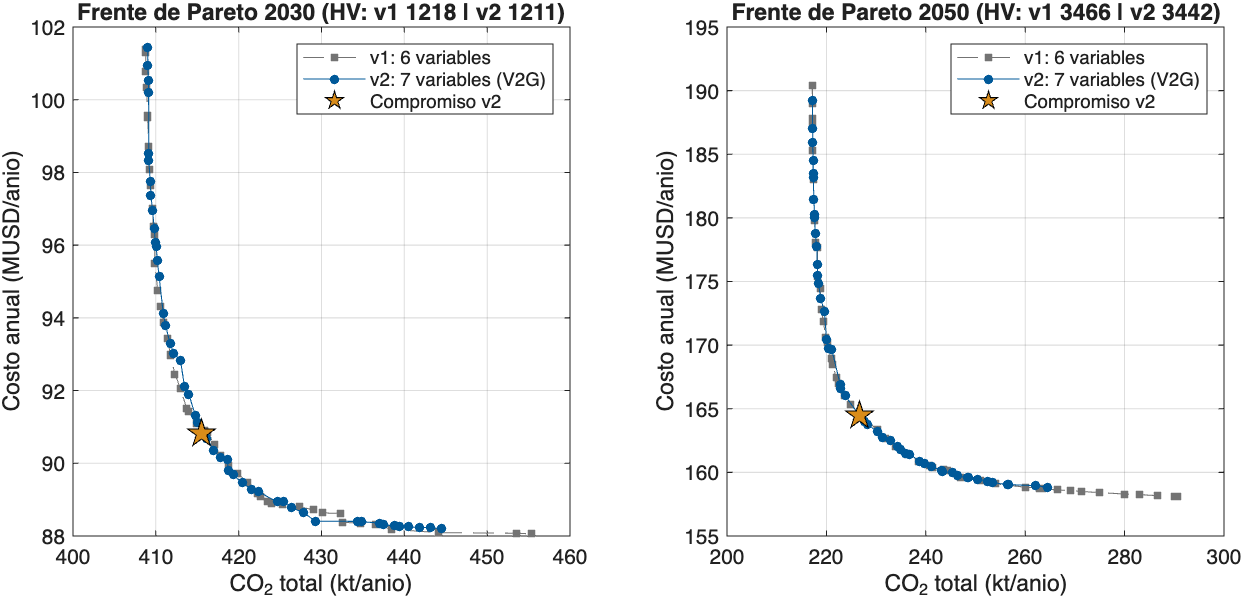
\includegraphics[width=\textwidth]{figs_v2/fig_v2_1_pareto.png}
\caption{Frentes de Pareto 2030 y 2050: versi\'on~1 (6 variables) frente a la versi\'on
vectorial (7 variables, con V2G). HV: hipervolumen respecto de un punto de referencia
com\'un.}
\label{fig:pareto}
\end{figure}

La huella vectorial $\bar{\vect{C}}$ (Figura~\ref{fig:hubC}) hace expl\'icita la
transici\'on: en 2024 el 74\% de la electricidad y el 72\% del agua dependen del SNI, y
el 99\% de la movilidad del combustible; en 2030 el SNI cae al 42\% (electricidad) y 34\%
(agua) mientras FV y e\'olica cubren 37--44\%; en 2050 la movilidad electrificada al 90\%
se alimenta 40\% de FV ---las horas diurnas de carga inteligente coinciden con el recurso
solar--- y s\'olo 18\% del SNI. Obs\'ervese que el vector agua est\'a sistem\'aticamente
\emph{m\'as} descarbonizado que la electricidad pura porque el bombeo diferible se
desplaza hacia las horas renovables: el acoplamiento agua--electricidad es el que primero
captura el excedente FV. El vector agua representa menos del 1\% de la energ\'ia y del
costo (Figura~\ref{fig:vectores}), pero su flexibilidad (tanques) es la m\'as barata del
sistema; el vector movilidad concentra el 71\% de las emisiones en 2030 y su
electrificaci\'on explica el 78\% de la reducci\'on 2030$\to$2050.

\begin{figure}[htbp]
\centering
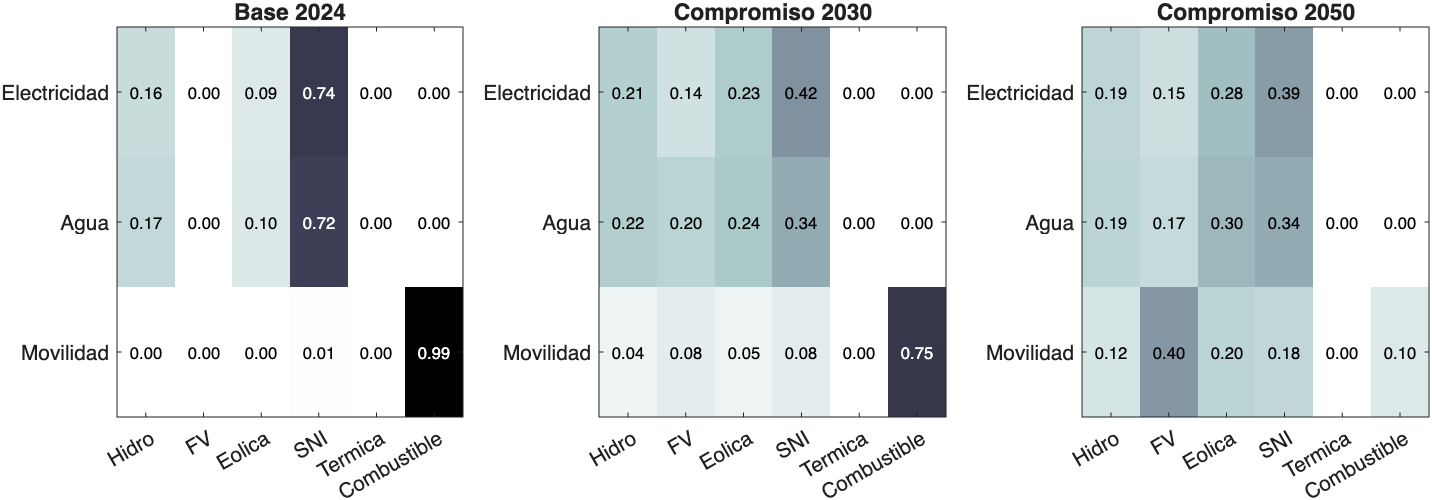
\includegraphics[width=\textwidth]{figs_v2/fig_v2_2_hub_C.png}
\caption{Matriz de acoplamiento media $\bar{\vect{C}}$ (fracci\'on de cada servicio
cubierta por cada portador) para la l\'inea base y las soluciones de compromiso.}
\label{fig:hubC}
\end{figure}

\begin{figure}[htbp]
\centering
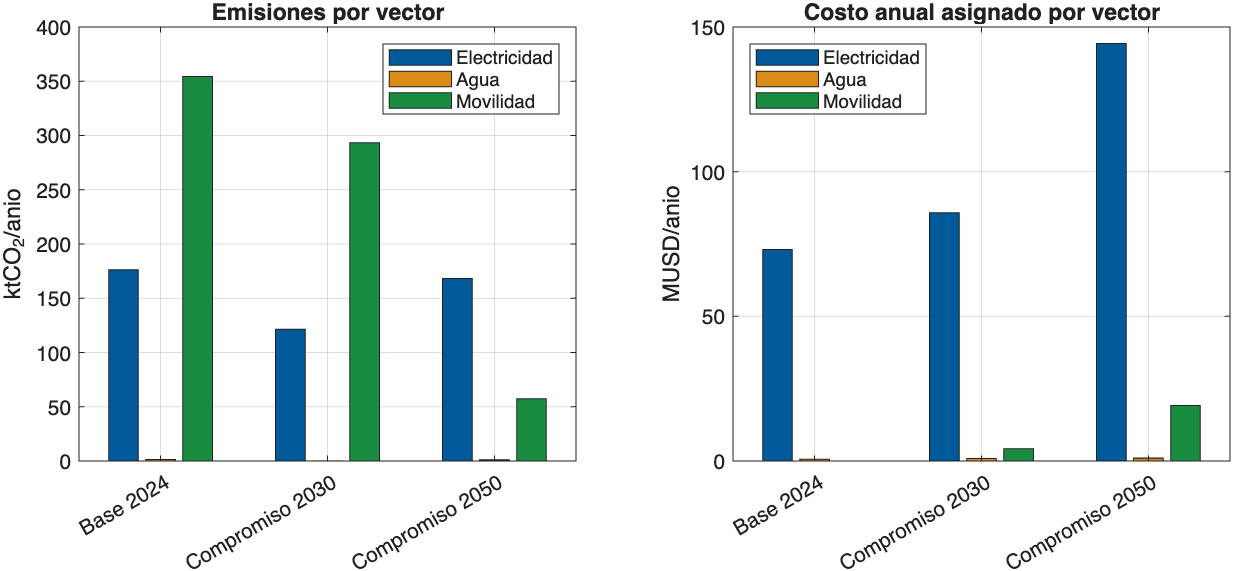
\includegraphics[width=0.95\textwidth]{figs_v2/fig_v2_3_vectores.png}
\caption{Emisiones y costo anual asignados por vector.}
\label{fig:vectores}
\end{figure}

\begin{figure}[htbp]
\centering
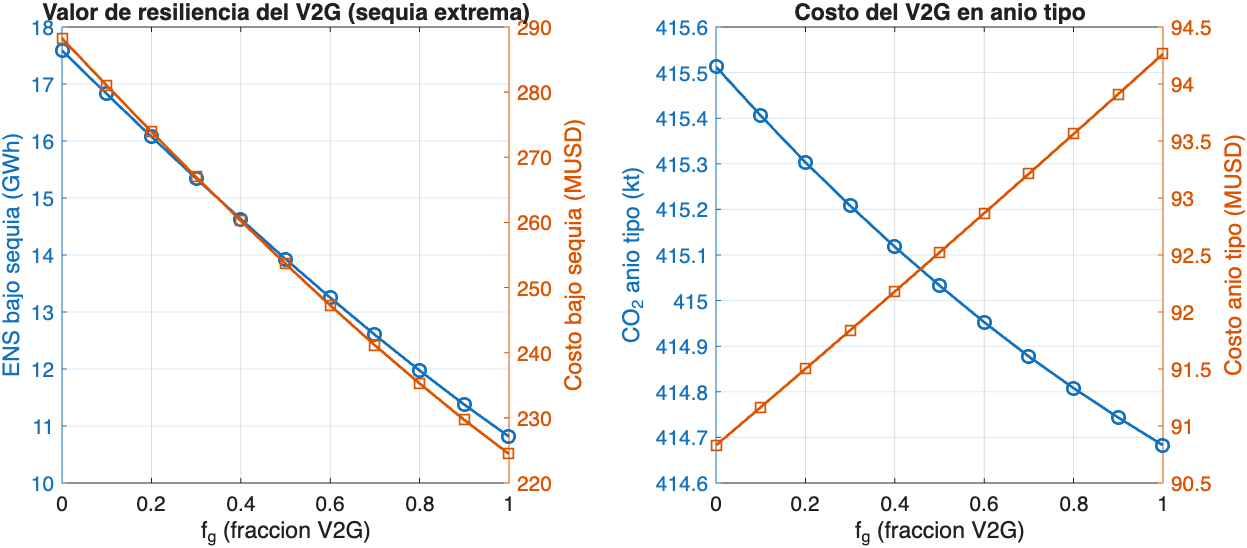
\includegraphics[width=\textwidth]{figs_v2/fig_v2_4_v2g.png}
\caption{Sensibilidad a la fracci\'on V2G $f_g$ para la soluci\'on de compromiso 2030:
valor bajo sequ\'ia extrema (izq.) y costo en el a\~no tipo (der.).}
\label{fig:v2g}
\end{figure}

\subsection{Autoencoder de escenarios}
Con 8 dimensiones latentes el autoencoder reconstruye los d\'ias de prueba con NRMSE de
2,8\% (demanda), 10,4\% (e\'olica) y 1,1\% (hidro), id\'entico a PCA (2,7\%, 10,4\%,
1,0\%), pero peor en FV (16,3\% vs.\ 8,2\%) (Tabla~\ref{tab:ae}, Figura~\ref{fig:ae}).
El resultado es esperable: los perfiles sint\'eticos de la
versi\'on~1 se generan por productos de formas diarias, factores mensuales y ruido
gaussiano, una estructura casi lineal en la que PCA es cercana al \'optimo y explica el
96,4\% de la varianza con 8 componentes. La ventaja del autoencoder no est\'a en la
compresi\'on sino en la \textbf{generaci\'on}: el muestreo latente jer\'arquico produce
a\~nos sint\'eticos cuya distribuci\'on de resultados, evaluados con \texttt{renon\_hub} sobre la
soluci\'on de compromiso 2030 de la versi\'on~1 (\CO\ mediana 417,8~kt, P5--P95
401--435; costo 90,2~MUSD, 83--98), coincide con la del Monte Carlo param\'etrico (422,7~kt,
400--443; 92,1~MUSD, 82--101) sin haber especificado ninguna distribuci\'on de
perturbaciones: la variabilidad interanual emerge de los datos. El espacio latente
muestra separabilidad estacional (varianza entre meses / total $=0{,}22$ en $z_1$). Con
las series reales de CENTROSUR, ETAPA y el recurso medido (PT1), donde las
no linealidades (nubosidad, r\'egimen de lluvias, feriados) s\'i son relevantes, se espera
que el autoencoder supere a PCA; ese contraste es una prueba de aceptaci\'on propuesta
para el Sprint~5.

\begin{table}[htbp]
\centering\small
\caption{Reconstrucci\'on de d\'ias de prueba (NRMSE, \%) con 8 dimensiones latentes.}
\label{tab:ae}
\begin{tabular}{lcccc}
\toprule
 & Demanda & FV & E\'olica & Hidro \\
\midrule
Autoencoder 96--64--8--64--96 & 2,77 & 16,27 & 10,42 & 1,09 \\
PCA (8 componentes, 96,4\% var.) & 2,75 & 8,20 & 10,41 & 1,01 \\
\bottomrule
\end{tabular}
\end{table}

\begin{figure}[htbp]
\centering
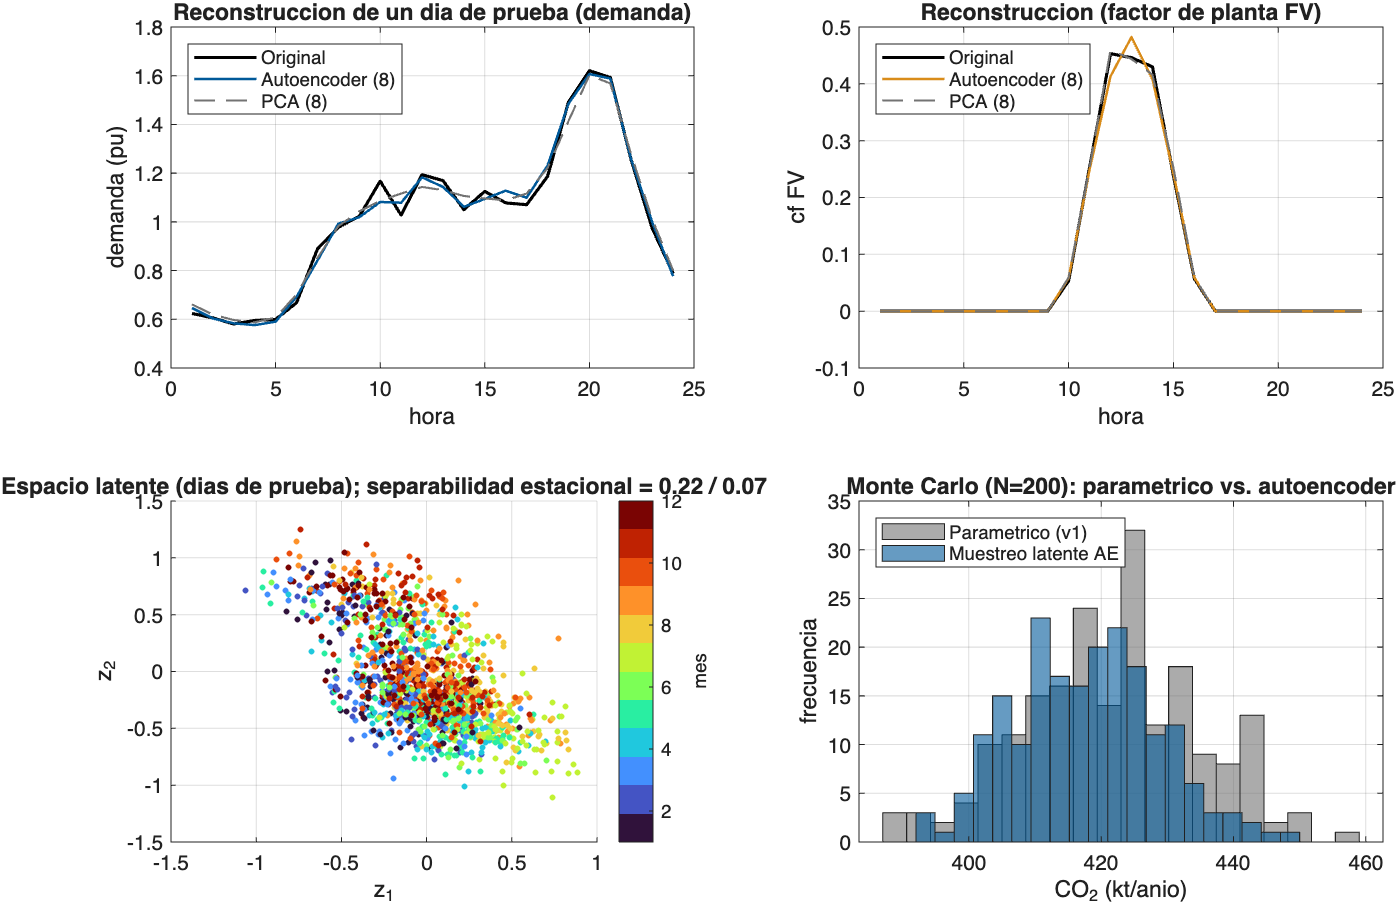
\includegraphics[width=\textwidth]{figs_v2/fig_v2_5_autoencoder.png}
\caption{Autoencoder de escenarios: reconstrucci\'on de un d\'ia de prueba (arriba),
espacio latente coloreado por mes (abajo izq.) y Monte Carlo del modelo hub con a\~nos
generados por muestreo latente frente al Monte Carlo param\'etrico (abajo der.).}
\label{fig:ae}
\end{figure}

\subsection{Modelos sustitutos: KAN, MLP y atenci\'on}
\label{sec:surr}
Los tres sustitutos aproximan el modelo hub con precisi\'on suficiente para
optimizaci\'on (Tabla~\ref{tab:surr}, Figura~\ref{fig:surr}): errores de 0,3--0,7~kt\CO\ y
0,3--0,7~MUSD sobre rangos de 100~kt y 70~MUSD. La KAN alcanza $R^2=0{,}9998$ en \CO\ con
\textbf{3,5 veces menos par\'ametros} que el MLP y 4,5 veces menos que el modelo de
atenci\'on, aunque es la menos precisa en costo ($R^2=0{,}995$; los puntos de mayor costo,
con bater\'ia grande, quedan fuera de la malla de splines) y la m\'as costosa de entrenar
en nuestra implementaci\'on no optimizada (38~s). El sustituto de atenci\'on es el m\'as
preciso en ambos objetivos.

\begin{table}[htbp]
\centering\small
\caption{Sustitutos del modelo hub (2030), 480 muestras de entrenamiento y 120 de prueba. Los tiempos de entrenamiento $t$ corresponden a una ejecuci\'on en MATLAB R2026a (Apple Silicon) y var\'ian entre ejecuciones; las m\'etricas de error son reproducibles con las semillas fijas.}
\label{tab:surr}
\begin{tabular}{lrrrrrr}
\toprule
\textbf{Modelo} & \textbf{Par\'am.} & \textbf{$t$ (s)} & \textbf{RMSE \CO} & \textbf{RMSE costo} & \textbf{$R^2$ \CO} & \textbf{$R^2$ costo} \\
\midrule
KAN $[7,6,2]$, $G=5$, $k=3$ & 486 & 38 & 0,33 kt & 0,66 MUSD & 0,9998 & 0,9953 \\
MLP $[7,32,32,2]$ & 1378 & 7 & 0,36 kt & 0,36 MUSD & 0,9997 & 0,9987 \\
Auto-atenci\'on ($d=8$) & 2194 & 34 & 0,30 kt & 0,28 MUSD & 0,9998 & 0,9992 \\
\bottomrule
\end{tabular}
\end{table}

\begin{figure}[htbp]
\centering
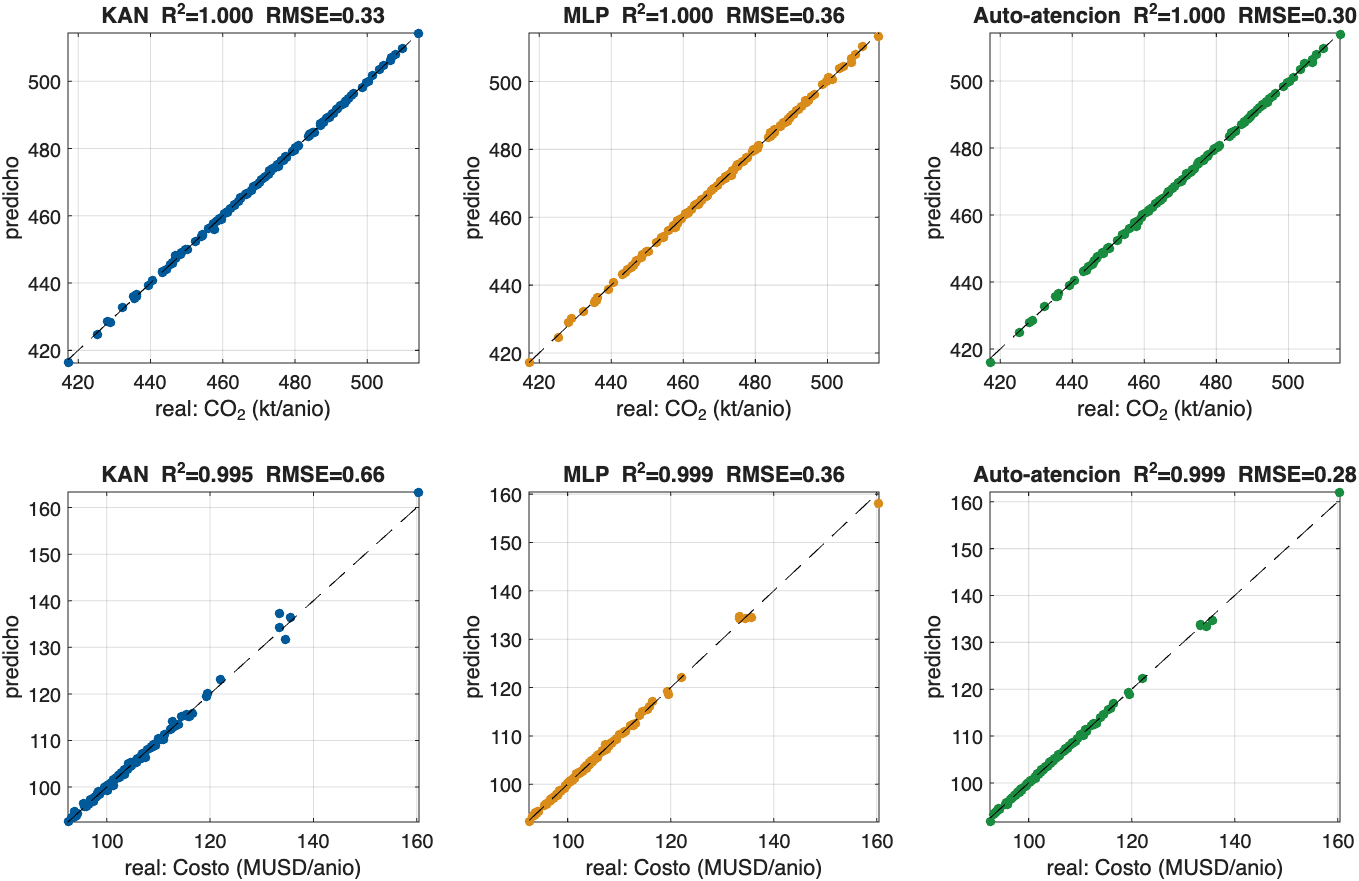
\includegraphics[width=\textwidth]{figs_v2/fig_v2_6_surrogates.png}
\caption{Predicci\'on frente a valor real en el conjunto de prueba para los tres sustitutos.}
\label{fig:surr}
\end{figure}

\paragraph{Interpretabilidad.} Las funciones $\phi_{1j}\ldots\phi_{7j}$ de la primera
capa de la KAN (Figura~\ref{fig:kan}) y su desviaci\'on est\'andar como medida de
importancia ordenan las variables: carga inteligente $f_v$ (29\%), e\'olica $P_w$ (24\%),
FV $P_{pv}$ (16\%), mini-hidro $P_h^+$ (14\%), V2G $f_g$ (9\%), bater\'ia $E_b$ (7\%) y
bombeo diferible $f_a$ (1\%). Las funciones de $f_v$ y $P_w$ son mon\'otonas y casi
lineales (efecto proporcional), la de $E_b$ es fuertemente no lineal en una sola arista
(la bater\'ia s\'olo importa a trav\'es del costo) y las de $f_a$ son planas (el bombeo es
demasiado peque\~no para mover los objetivos), lo que coincide con la lectura de la
Tabla~\ref{tab:vec}. El mapa de auto-atenci\'on (Figura~\ref{fig:attmap}) es
consistente: la fila y la columna de $f_v$ concentran los pesos (autoatenci\'on 0,35;
$f_a\to f_v$ 0,25), es decir, el modelo aprende que las interacciones relevantes pasan
por la carga inteligente, y $P_h^+$ atiende sobre todo a $P_{pv}$ (0,21), reflejando la
complementariedad diaria hidro--solar.

\begin{figure}[htbp]
\centering
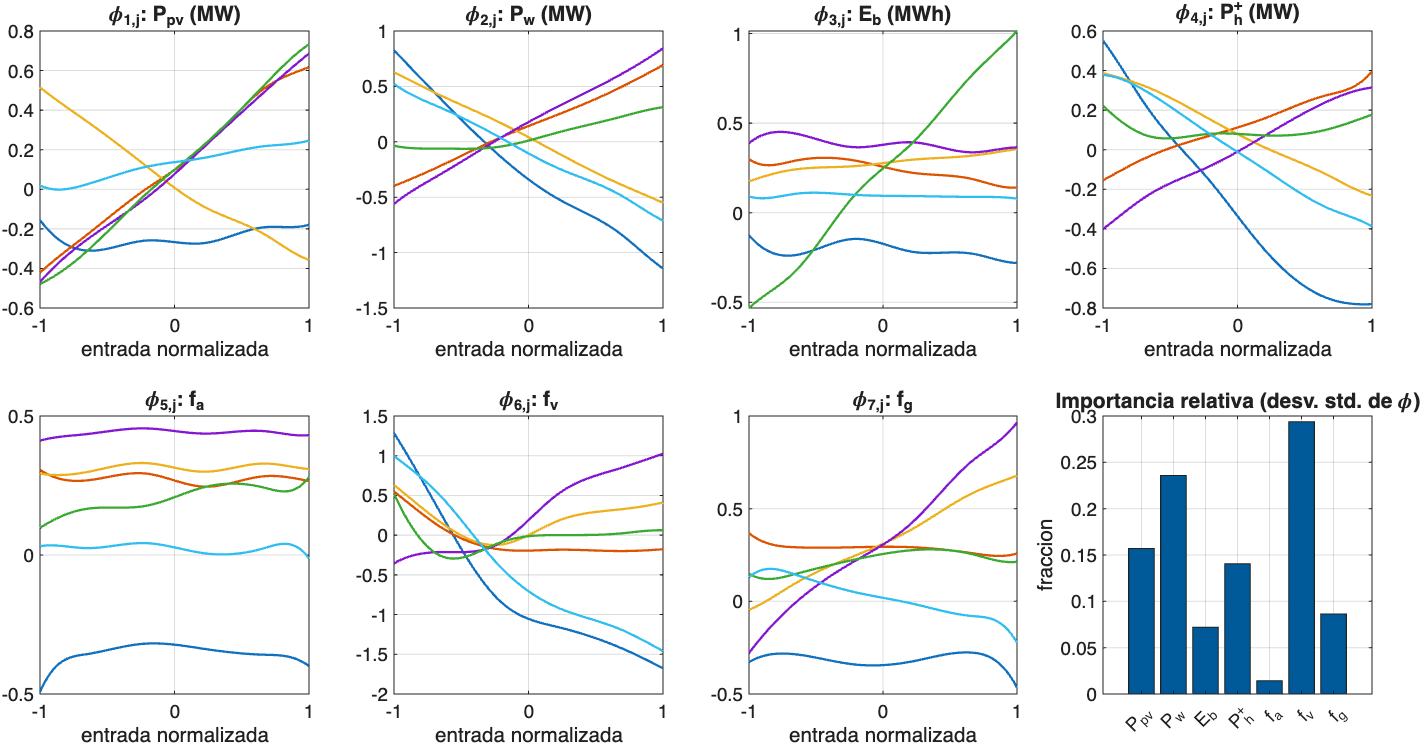
\includegraphics[width=\textwidth]{figs_v2/fig_v2_8_kan_activaciones.png}
\caption{Funciones de activaci\'on aprendidas en las aristas de la primera capa de la KAN
(una curva por neurona oculta) e importancia relativa de cada variable de decisi\'on.}
\label{fig:kan}
\end{figure}

\begin{figure}[htbp]
\centering
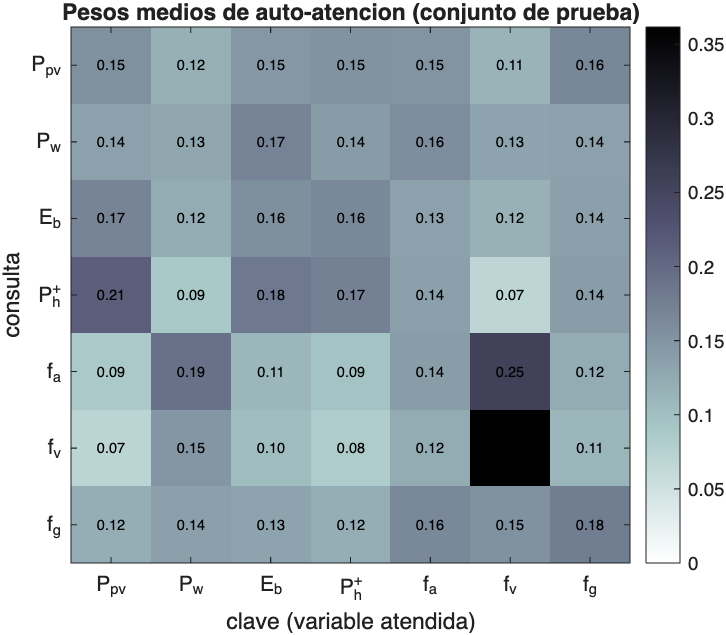
\includegraphics[width=0.6\textwidth]{figs_v2/fig_v2_9_atencion_mapa.png}
\caption{Pesos medios de auto-atenci\'on entre variables de decisi\'on (conjunto de prueba).}
\label{fig:attmap}
\end{figure}

\paragraph{Optimizaci\'on asistida.} NSGA-II ejecutado sobre la KAN y re-evaluado con el
modelo completo recupera el \textbf{94,7\% del hipervolumen} del frente real (948 vs.\
1001) con 648 evaluaciones reales (600 de entrenamiento $+$ 48 de re-evaluaci\'on) en lugar
de 2928, un ahorro del 78\% (Figura~\ref{fig:nsgakan}). En el modelo hub, cuyo costo por
evaluaci\'on es de milisegundos, el tiempo total es mayor por el entrenamiento; pero
proyectado al modelo EnergyPLAN de Trento (4,3~s por evaluaci\'on~\cite{loza2026}) el
ahorro equivaldr\'ia a 2,7~h por corrida, y en los modelos con restricciones de red y
Monte Carlo del PT3 la ventaja escala linealmente. El sesgo observado (el frente asistido
queda 1--2~MUSD por encima en la zona intermedia) se corrige con el esquema est\'andar de
re-entrenamiento incremental~\cite{jin2011} o con la optimizaci\'on bayesiana ya
validada en~\cite{loza2026}.

\begin{figure}[htbp]
\centering
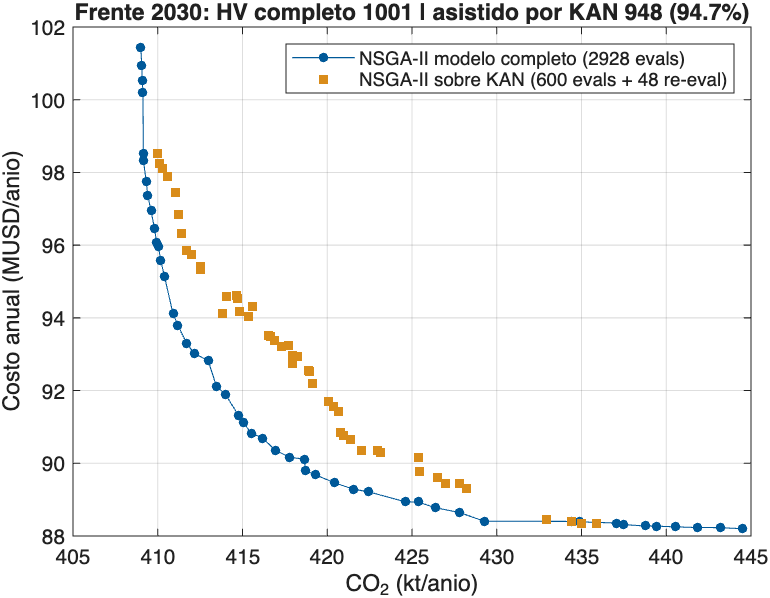
\includegraphics[width=0.62\textwidth]{figs_v2/fig_v2_10_nsga_kan.png}
\caption{Frente 2030 con el modelo completo frente al frente obtenido sobre el sustituto
KAN y re-evaluado con el modelo completo.}
\label{fig:nsgakan}
\end{figure}

\subsection{Dream Optimization Algorithm}
En el problema restringido (costo m\'inimo con $J_1\le415$~kt), con presupuesto de 3000
evaluaciones y 6 semillas, DOA obtiene $J=90{,}86\pm0{,}10$~MUSD, estad\'isticamente
equivalente a PSO ($90{,}80\pm0{,}001$) y mejor que GA ($93{,}38\pm1{,}72$) y que la
b\'usqueda aleatoria ($100{,}2\pm3{,}5$) (Tabla~\ref{tab:doa}, Figura~\ref{fig:doaconv}).
La mejor soluci\'on DOA (283--287~MW FV, 150~MW e\'olica, sin bater\'ia, 30~MW mini-hidro,
$f_v=0{,}74$, $f_g=0$; \CO\ $=415{,}0$~kt, costo 90,81~MUSD) coincide con la del frente
NSGA-II en ese nivel de emisiones, lo que confirma la consistencia entre m\'etodos. DOA
converge m\'as r\'apido que GA (alcanza 91~MUSD en $\approx$700 evaluaciones frente a
$>$3000 de GA) y con menor dispersi\'on entre semillas que GA, aunque PSO lo iguala en
este problema suave de 7 variables; la ventaja de DOA reportada por sus autores se
manifiesta en problemas multimodales de mayor dimensi\'on~\cite{lang2025}, como ser\'an
los del PT3 (escenarios urbano/rural con decenas de variables).

\begin{table}[htbp]
\centering\small
\caption{Problema mono-objetivo restringido (2030): estad\'isticas sobre 6 semillas, 3000 evaluaciones.}
\label{tab:doa}
\begin{tabular}{lrrrr}
\toprule
\textbf{Algoritmo} & \textbf{$J$ media} & \textbf{desv.\ est.} & \textbf{$J$ m\'in.} & \textbf{$J$ m\'ax.} \\
\midrule
DOA (reimplementaci\'on) & 90,86 & 0,096 & 90,81 & 91,05 \\
GA (\emph{Global Optimization Toolbox}) & 93,38 & 1,717 & 91,70 & 95,52 \\
PSO (\emph{Global Optimization Toolbox}) & 90,80 & 0,001 & 90,79 & 90,80 \\
B\'usqueda aleatoria & 100,25 & 3,478 & 95,11 & 104,22 \\
\bottomrule
\end{tabular}
\end{table}

\begin{figure}[htbp]
\centering
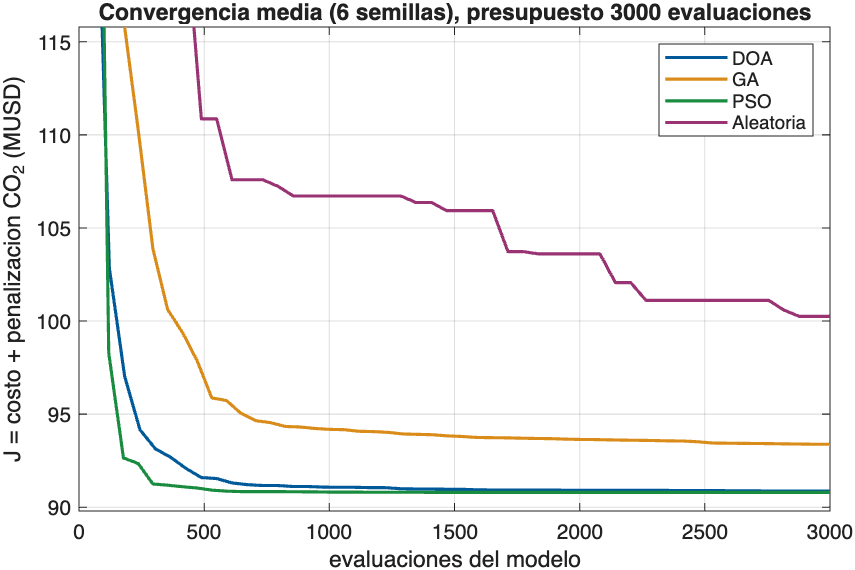
\includegraphics[width=0.66\textwidth]{figs_v2/fig_v2_11_doa_convergencia.png}
\caption{Convergencia media de los cuatro algoritmos (6 semillas).}
\label{fig:doaconv}
\end{figure}

En la construcci\'on del frente por escalarizaci\'on de Tchebycheff, 12 corridas
independientes de DOA (3168 evaluaciones en total) alcanzan el \textbf{95,3\% del
hipervolumen} de NSGA-II (1047 vs.\ 1099 con 2928 evaluaciones), Figura~\ref{fig:doafront}.
Los puntos DOA se ubican sobre el frente en la zona de bajo costo y presentan
dispersi\'on en la zona de bajo \CO, donde la escalarizaci\'on con presupuesto peque\~no
(264 evaluaciones por peso) converge parcialmente. Este resultado sugiere un uso pr\'actico
del DOA en el proyecto: \textbf{refinamiento local} de soluciones de inter\'es del frente
(p.ej.\ la de compromiso) y \textbf{sintonizaci\'on de hiperpar\'ametros} del EMS, tareas
mono-objetivo en las que su simplicidad (sin operadores de cruce ni par\'ametros de
inercia) es una ventaja.

\begin{figure}[htbp]
\centering
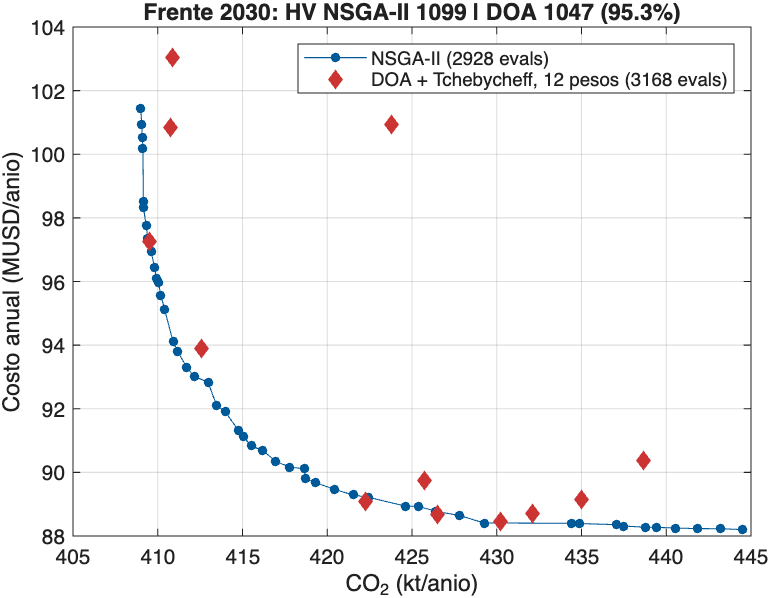
\includegraphics[width=0.62\textwidth]{figs_v2/fig_v2_12_doa_frente.png}
\caption{Frente 2030: NSGA-II frente a DOA con escalarizaci\'on de Tchebycheff (12 pesos).}
\label{fig:doafront}
\end{figure}

\subsection{EMS con atenci\'on temporal}
La Tabla~\ref{tab:ems} compara, para la soluci\'on de compromiso 2030 de la versi\'on~1
(255~MW FV, 150~MW e\'olica, 30~MW mini-hidro, $f_a=0{,}33$, $f_v=0{,}84$), el llenado de
valles con la atenci\'on temporal antes y despu\'es de sintonizar $\theta$ con DOA (320
evaluaciones). Con las se\~nales del a\~no tipo (factor de emisi\'on y precio del SNI con
variaci\'on mensual y ruido) la atenci\'on sintonizada iguala al llenado de valles
(\CO\ 417,7 vs.\ 417,8~kt; costo 90,10 vs.\ 90,22~MUSD, $-0{,}13\%$) y la resiliencia bajo
sequ\'ia es id\'entica (ENS 10,99~GWh); con par\'ametros no sintonizados es ligeramente
peor ($+0{,}4\%$ en \CO). Se construy\'o adem\'as un escenario con \textbf{tarifa horaria}
(valle 0--6~h $\times0{,}7$, punta 18--22~h $\times1{,}6$) y \textbf{factor de emisi\'on
marginal horario} (mediod\'ia $\times0{,}8$, punta $\times1{,}4$): la ganancia sigue
siendo marginal ($-0{,}23\%$ en costo, $+0{,}07\%$ en \CO). La explicaci\'on es
cuantitativa: la energ\'ia flexible es s\'olo el 4\% de la demanda anual (bombeo diferible
4~GWh $+$ carga inteligente 65~GWh) y el llenado de valles ya la sit\'ua en las horas
nocturnas, que coinciden con el valle tarifario; el margen de mejora es peque\~no por
construcci\'on. El resultado es \'util en dos sentidos: (i)~valida que la heur\'istica de
la versi\'on~1 es casi \'optima para el caso actual, y (ii)~deja lista una pol\'itica
parametrizada y sintonizable que \emph{generaliza} el llenado de valles y cuyo beneficio
crecer\'a con la penetraci\'on de VE (2050: 327~GWh de movilidad), con tarifas horarias
reales de ARCERNNR y con se\~nales de red (congesti\'on de alimentadores) que el llenado
de valles no puede incorporar.

\begin{table}[htbp]
\centering\small
\caption{EMS: llenado de valles frente a atenci\'on temporal (soluci\'on de compromiso 2030 de la versi\'on~1).}
\label{tab:ems}
\begin{tabular}{llrrrr}
\toprule
\textbf{Se\~nales} & \textbf{EMS} & \textbf{\CO\ (kt)} & \textbf{Costo (MUSD)} & \textbf{Import.\ (GWh)} & \textbf{ENS sequ\'ia (GWh)} \\
\midrule
\multirow{3}{*}{A\~no tipo}
 & Llenado de valles & 417,76 & 90,22 & 690,2 & 10,99 \\
 & Atenci\'on ($\theta$ por defecto) & 419,42 & 90,84 & 702,5 & 11,36 \\
 & Atenci\'on sintonizada (DOA) & 417,71 & 90,10 & 690,1 & 10,99 \\
\midrule
\multirow{3}{*}{Tarifa y FE horarios}
 & Llenado de valles & 436,73 & 101,52 & 690,2 & -- \\
 & Atenci\'on ($\theta$ por defecto) & 436,80 & 101,47 & 691,2 & -- \\
 & Atenci\'on sintonizada (DOA) & 437,05 & 101,29 & 690,5 & -- \\
\bottomrule
\end{tabular}
\end{table}

\begin{figure}[htbp]
\centering
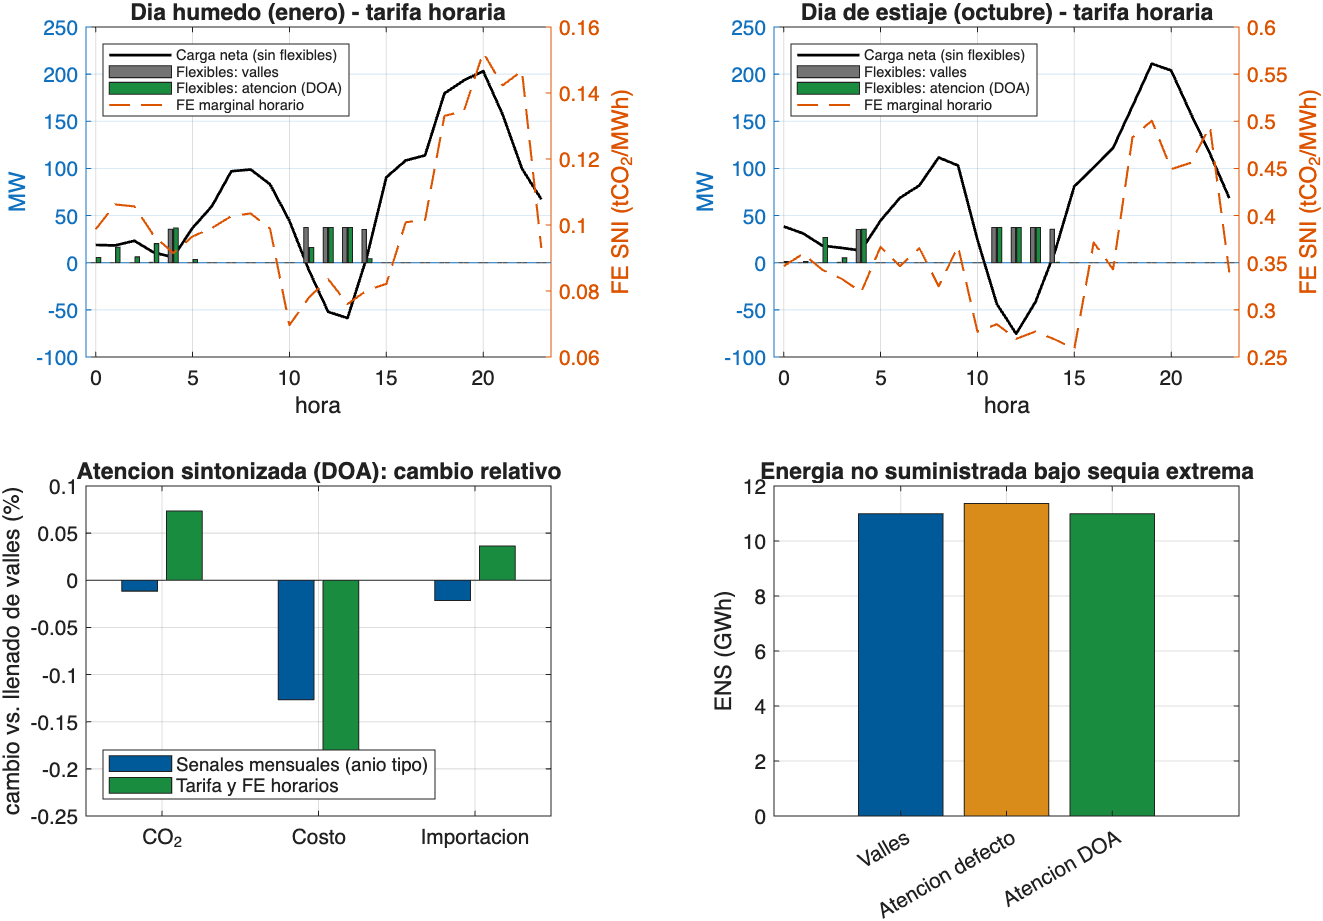
\includegraphics[width=\textwidth]{figs_v2/fig_v2_13_ems_atencion.png}
\caption{EMS con atenci\'on temporal: asignaci\'on de cargas flexibles en un d\'ia
h\'umedo y uno de estiaje con tarifa horaria (arriba), cambio relativo frente al llenado
de valles (abajo izq.) y ENS bajo sequ\'ia extrema (abajo der.).}
\label{fig:ems}
\end{figure}

%=====================================================================
\section{Discusi\'on: flujo de trabajo propuesto para el entregable PT2}
%=====================================================================
Los experimentos permiten fijar, con evidencia, la arquitectura del EMS y de la cadena
de planificaci\'on que se publicar\'a en GitHub en febrero de 2027:
\begin{enumerate}[leftmargin=1.6em]
  \item \textbf{Datos $\to$ escenarios.} Base de datos PT1 (CENTROSUR, ETAPA, ANT/EMOV,
  recurso) $\to$ autoencoder de d\'ias $\to$ generador latente jer\'arquico. Criterio de
  aceptaci\'on: NRMSE $<15\%$ y Pearson $>0{,}85$ frente a mediciones (Formulario~2) y
  NRMSE del autoencoder $\le$ PCA en todas las variables con datos reales.
  \item \textbf{Modelo vectorial.} \texttt{renon\_hub} calibrado; salida est\'andar:
  objetivos, $\bar{\vect{C}}$, indicadores por vector y $\kappa$. Extensi\'on inmediata:
  restricciones de red de distribuci\'on y separaci\'on urbano/rural (Tarqui, Victoria del
  Portete, Cumbe).
  \item \textbf{Sustituto.} KAN como sustituto \emph{interpretable} para an\'alisis de
  sensibilidad y talleres con actores (las curvas $\phi_{ij}$ son comunicables a
  CENTROSUR/ETAPA); MLP o atenci\'on como sustituto de \emph{precisi\'on} dentro del
  optimizador; re-entrenamiento incremental.
  \item \textbf{Optimizaci\'on.} NSGA-II (referencia) y optimizaci\'on bayesiana qNEHVI
  para el frente~\cite{daulton2021,loza2026}; DOA para refinamiento local y para
  sintonizar el EMS; tercer objetivo o restricci\'on de resiliencia (ENS bajo sequ\'ia)
  para valorar V2G y almacenamiento.
  \item \textbf{Operaci\'on.} EMS jer\'arquico con pol\'itica de atenci\'on temporal
  sintonizada por escenario tarifario; l\'inea base de llenado de valles como control.
  \item \textbf{Validaci\'on (PT4).} M\'etricas NRMSE/Pearson y comparaci\'on con los
  casos de Dinamarca, Alemania e Italia (Trento ya replicado).
\end{enumerate}

\paragraph{Limitaciones.} (i)~Todos los resultados usan perfiles sint\'eticos y
par\'ametros provinciales estimados; los valores absolutos cambiar\'an con la
calibraci\'on del PT1. (ii)~La KAN y el DOA son reimplementaciones propias, no las
bibliotecas de los autores; los hiperpar\'ametros no fueron optimizados. (iii)~El
autoencoder se evalu\'o con una sola arquitectura y semilla. (iv)~El V2G se model\'o con
una ventana fija y sin degradaci\'on dependiente de la profundidad de descarga.
(v)~Las comparaciones de tiempo de c\'omputo no son concluyentes para un modelo de
milisegundos por evaluaci\'on; su lectura correcta es en n\'umero de evaluaciones.

%=====================================================================
\section{Plan de trabajo extendido (Sprints 4--8)}
%=====================================================================
\begin{table}[htbp]
\centering\small
\caption{Actividades propuestas para el PT2 con base en este reporte.}
\label{tab:plan}
\begin{tabular}{p{1.9cm}p{7.2cm}p{2.2cm}p{2.6cm}}
\toprule
\textbf{Sprint} & \textbf{Actividad} & \textbf{Responsable} & \textbf{Producto} \\
\midrule
4 (oct 2026) & Calibraci\'on de \texttt{renon\_hub} con series reales; validaci\'on NRMSE/Pearson; autoencoder vs.\ PCA con datos reales & TINV, INV2, AI & Reporte de calibraci\'on \\
5 (nov 2026) & Restricciones de red y partici\'on urbano/rural; tercer objetivo de resiliencia; V2G con degradaci\'on & TINV, INV1 & \texttt{renon\_hub} v3 \\
6 (dic 2026) & Sustituto KAN/atenci\'on con re-entrenamiento incremental; qNEHVI en MATLAB o Python (BoTorch) & TINV, INV1 & M\'odulo de optimizaci\'on \\
7 (ene 2027) & EMS de atenci\'on con tarifas ARCERNNR y se\~nales de red; sintonizaci\'on DOA; pruebas en supercomputador DEET & TINV, DP & EMS documentado \\
8 (feb 2027) & Documentaci\'on, pruebas unitarias, licencia MIT, publicaci\'on en GitHub; sesi\'on de retroalimentaci\'on con actores & TINV, DP, INV2 & \textbf{Entregable PT2} \\
\bottomrule
\end{tabular}
\end{table}

%=====================================================================
\section{Conclusiones}
%=====================================================================
\begin{enumerate}[leftmargin=1.6em]
  \item La formulaci\'on vectorial (concentrador energ\'etico) del modelo ReNoN es
  compatible con la versi\'on~1 ---la reproduce exactamente--- y a\~nade la huella
  vectorial $\bar{\vect{C}}$, los indicadores por vector y el \'indice de acoplamiento
  $\kappa$, que hacen legible la transici\'on: el SNI pasa de cubrir el 74\% de la
  electricidad en 2024 al 42\% en 2030 y al 39\% en 2050, y la movilidad electrificada de
  2050 se alimenta 40\% de FV.
  \item El V2G no es seleccionado por el optimizador en el a\~no tipo con los costos
  asumidos, pero reduce 38\% la energ\'ia no suministrada bajo sequ\'ia extrema; su
  valoraci\'on exige objetivos expl\'icitos de resiliencia.
  \item Los sustitutos KAN, MLP y de atenci\'on reproducen el modelo con $R^2\ge0{,}995$; la
  KAN lo hace con 486 par\'ametros y ofrece curvas de sensibilidad interpretables que
  identifican la carga inteligente de VE y la e\'olica como las palancas dominantes. La
  optimizaci\'on asistida por KAN recupera el 94,7\% del hipervolumen con 78\% menos
  evaluaciones.
  \item El DOA, reimplementado a partir de su descripci\'on publicada, iguala a PSO y
  supera a GA en el problema restringido y reconstruye el 95\% del hipervolumen de NSGA-II
  por escalarizaci\'on; su nicho en el proyecto es el refinamiento local y la
  sintonizaci\'on del EMS.
  \item El autoencoder no supera a PCA en compresi\'on de los perfiles sint\'eticos
  (casi lineales) pero provee un generador de escenarios libre de supuestos
  distribucionales cuya salida coincide con el Monte Carlo param\'etrico.
  \item El EMS con atenci\'on temporal generaliza el llenado de valles; con la carga
  flexible actual (4\% de la demanda) su ganancia es marginal ($\le0{,}3\%$), lo que
  valida la heur\'istica de la versi\'on~1 y acota el beneficio esperable a escenarios con
  mayor electrificaci\'on y tarifas horarias.
\end{enumerate}

%---------------------------------------------------------------------
% Bibliografia del reporte tecnico v2 (ReNoN-Azuay)
%---------------------------------------------------------------------
\begin{thebibliography}{99}

\bibitem{formulario2} GIEEC--DEET, ``Formulario 2: Propuesta de proyecto v2 ---
Transici\'on energ\'etica sostenible en Azuay--Ecuador mediante infraestructuras
integradas,'' XXII Concurso Universitario de Proyectos de Investigaci\'on, VIUC,
Universidad de Cuenca, ene.~2026.

\bibitem{reporte_v1} GIEEC--DEET, ``Propuesta t\'ecnica de soluci\'on: modelo
multivectorial ReNoN para la transici\'on energ\'etica sostenible en Azuay--Ecuador.
Reporte t\'ecnico de dise\~no, implementaci\'on y simulaci\'on en MATLAB (v1),''
Universidad de Cuenca, jul.~2026. Disponible en
\url{https://github.com/ismael-minchala/renon-azuay}.

\bibitem{ortega2026} M.~Ortega Ortega, L.~I.~Minchala y P.~Ar\'evalo Cordero,
``Structural vulnerabilities and GHG emissions in Ecuador's electricity generation
(2003--2024): A diagnostic approach,'' \emph{Electronics}, vol.~15, no.~16, art.~3697,
2026. doi:\href{https://doi.org/10.3390/electronics15163697}{10.3390/electronics15163697}.

\bibitem{loza2026} B.~Loza, ``Replicaci\'on de la metodolog\'ia EnergyPLAN$+$MOEA y
optimizaci\'on bayesiana para la planificaci\'on 2030/2050 (caso Trento),'' Reporte de
avance PT2, Proyecto ReNoN--Azuay, Universidad de Cuenca, sep.~2026.

\bibitem{viesi2020} D.~Viesi, L.~Crema, M.~S.~Mahbub, A.~Verones, R.~Brunelli,
P.~Baggio, M.~Fauri, D.~Prada, A.~Bello, B.~Nodari, S.~Silvestri y M.~Tomasi,
``Integrated and dynamic energy modelling of a regional system: A cost-optimized
approach in the deep decarbonisation of the Province of Trento (Italy),''
\emph{Energy}, vol.~209, art.~118378, 2020.
doi:\href{https://doi.org/10.1016/j.energy.2020.118378}{10.1016/j.energy.2020.118378}.

\bibitem{lund2021} H.~Lund, J.~Z.~Thellufsen, P.~A.~{\O}stergaard, P.~Sorkn{\ae}s,
I.~R.~Skov y B.~V.~Mathiesen, ``EnergyPLAN -- Advanced analysis of smart energy
systems,'' \emph{Smart Energy}, vol.~1, art.~100007, 2021.
doi:\href{https://doi.org/10.1016/j.segy.2021.100007}{10.1016/j.segy.2021.100007}.

\bibitem{geidl2007hub} M.~Geidl, G.~Koeppel, P.~Favre-Perrod, B.~Kl\"ockl,
G.~Andersson y K.~Fr\"ohlich, ``Energy hubs for the future,'' \emph{IEEE Power and
Energy Magazine}, vol.~5, no.~1, pp.~24--30, 2007.
doi:\href{https://doi.org/10.1109/MPAE.2007.264850}{10.1109/MPAE.2007.264850}.

\bibitem{geidl2007opf} M.~Geidl y G.~Andersson, ``Optimal power flow of multiple
energy carriers,'' \emph{IEEE Transactions on Power Systems}, vol.~22, no.~1,
pp.~145--155, 2007.
doi:\href{https://doi.org/10.1109/TPWRS.2006.888988}{10.1109/TPWRS.2006.888988}.

\bibitem{mancarella2014} P.~Mancarella, ``MES (multi-energy systems): An overview of
concepts and evaluation models,'' \emph{Energy}, vol.~65, pp.~1--17, 2014.
doi:\href{https://doi.org/10.1016/j.energy.2013.10.041}{10.1016/j.energy.2013.10.041}.

\bibitem{chicco2009} G.~Chicco y P.~Mancarella, ``Distributed multi-generation: A
comprehensive view,'' \emph{Renewable and Sustainable Energy Reviews}, vol.~13, no.~3,
pp.~535--551, 2009.
doi:\href{https://doi.org/10.1016/j.rser.2007.11.014}{10.1016/j.rser.2007.11.014}.

\bibitem{kempton2005} W.~Kempton y J.~Tomi\'c, ``Vehicle-to-grid power fundamentals:
Calculating capacity and net revenue,'' \emph{Journal of Power Sources}, vol.~144,
no.~1, pp.~268--279, 2005.
doi:\href{https://doi.org/10.1016/j.jpowsour.2004.12.022}{10.1016/j.jpowsour.2004.12.022}.

\bibitem{deb2002} K.~Deb, A.~Pratap, S.~Agarwal y T.~Meyarivan, ``A fast and elitist
multiobjective genetic algorithm: NSGA-II,'' \emph{IEEE Transactions on Evolutionary
Computation}, vol.~6, no.~2, pp.~182--197, 2002.
doi:\href{https://doi.org/10.1109/4235.996017}{10.1109/4235.996017}.

\bibitem{zitzler1999} E.~Zitzler y L.~Thiele, ``Multiobjective evolutionary
algorithms: A comparative case study and the strength Pareto approach,'' \emph{IEEE
Transactions on Evolutionary Computation}, vol.~3, no.~4, pp.~257--271, 1999.
doi:\href{https://doi.org/10.1109/4235.797969}{10.1109/4235.797969}.

\bibitem{lang2025} Y.~Lang y Y.~Gao, ``Dream Optimization Algorithm (DOA): A novel
metaheuristic optimization algorithm inspired by human dreams and its applications to
real-world engineering problems,'' \emph{Computer Methods in Applied Mechanics and
Engineering}, vol.~436, art.~117718, 2025.
doi:\href{https://doi.org/10.1016/j.cma.2024.117718}{10.1016/j.cma.2024.117718}.

\bibitem{daulton2021} S.~Daulton, M.~Balandat y E.~Bakshy, ``Parallel Bayesian
optimization of multiple noisy objectives with expected hypervolume improvement,''
en \emph{Advances in Neural Information Processing Systems 34 (NeurIPS 2021)}, 2021.
arXiv:\href{https://doi.org/10.48550/arXiv.2105.08195}{2105.08195}
(doi:10.48550/arXiv.2105.08195).

\bibitem{ozaki2020} Y.~Ozaki, Y.~Tanigaki, S.~Watanabe y M.~Onishi, ``Multiobjective
tree-structured Parzen estimator for computationally expensive optimization
problems,'' en \emph{Proc.\ Genetic and Evolutionary Computation Conference (GECCO
'20)}, pp.~533--541, 2020.
doi:\href{https://doi.org/10.1145/3377930.3389817}{10.1145/3377930.3389817}.

\bibitem{jin2011} Y.~Jin, ``Surrogate-assisted evolutionary computation: Recent
advances and future challenges,'' \emph{Swarm and Evolutionary Computation}, vol.~1,
no.~2, pp.~61--70, 2011.
doi:\href{https://doi.org/10.1016/j.swevo.2011.05.001}{10.1016/j.swevo.2011.05.001}.

\bibitem{mckay1979} M.~D.~McKay, R.~J.~Beckman y W.~J.~Conover, ``A comparison of
three methods for selecting values of input variables in the analysis of output from a
computer code,'' \emph{Technometrics}, vol.~21, no.~2, pp.~239--245, 1979.
doi:\href{https://doi.org/10.1080/00401706.1979.10489755}{10.1080/00401706.1979.10489755}.

\bibitem{liu2024kan} Z.~Liu, Y.~Wang, S.~Vaidya, F.~Ruehle, J.~Halverson,
M.~Solja\v{c}i\'c, T.~Y.~Hou y M.~Tegmark, ``KAN: Kolmogorov--Arnold Networks,'' en
\emph{International Conference on Learning Representations (ICLR 2025)}, 2025.
arXiv:\href{https://doi.org/10.48550/arXiv.2404.19756}{2404.19756}
(doi:10.48550/arXiv.2404.19756).

\bibitem{vaca2024} C.~J.~Vaca-Rubio, L.~Blanco, R.~Pereira y M.~Caus,
``Kolmogorov--Arnold Networks (KANs) for time series analysis,'' 2024.
arXiv:\href{https://doi.org/10.48550/arXiv.2405.08790}{2405.08790}
(doi:10.48550/arXiv.2405.08790).

\bibitem{hinton2006} G.~E.~Hinton y R.~R.~Salakhutdinov, ``Reducing the
dimensionality of data with neural networks,'' \emph{Science}, vol.~313, no.~5786,
pp.~504--507, 2006.
doi:\href{https://doi.org/10.1126/science.1127647}{10.1126/science.1127647}.

\bibitem{vaswani2017} A.~Vaswani, N.~Shazeer, N.~Parmar, J.~Uszkoreit, L.~Jones,
A.~N.~Gomez, {\L}.~Kaiser e I.~Polosukhin, ``Attention is all you need,'' en
\emph{Advances in Neural Information Processing Systems 30 (NeurIPS 2017)}, 2017.
arXiv:\href{https://doi.org/10.48550/arXiv.1706.03762}{1706.03762}
(doi:10.48550/arXiv.1706.03762).

\bibitem{zhou2021informer} H.~Zhou, S.~Zhang, J.~Peng, S.~Zhang, J.~Li, H.~Xiong y
W.~Zhang, ``Informer: Beyond efficient Transformer for long sequence time-series
forecasting,'' \emph{Proceedings of the AAAI Conference on Artificial Intelligence},
vol.~35, no.~12, pp.~11106--11115, 2021.
doi:\href{https://doi.org/10.1609/aaai.v35i12.17325}{10.1609/aaai.v35i12.17325}.

\end{thebibliography}


\vspace{1em}
\noindent\small\textit{Reproducibilidad: el c\'odigo MATLAB de esta versi\'on est\'a en
\texttt{code/analysis/propuesta\_tecnica/matlab\_v2/} del repositorio
\url{https://github.com/ismael-minchala/renon-azuay}. El script
\texttt{reproduce\_report\_v2} ejecuta en orden \texttt{s1\_hub}, \texttt{s2\_autoencoder},
\texttt{s3\_surrogates}, \texttt{s4\_doa} y \texttt{s5\_attention\_ems} con semillas fijas
(MATLAB R2026a; requiere Deep Learning, Optimization, Global Optimization y Statistics and
Machine Learning Toolbox; Parallel Computing Toolbox opcional). Las tablas CSV est\'an en
\texttt{resultados\_v2/}, las figuras en \texttt{reporte/figs\_v2/} y las pruebas de
regresi\'on en \texttt{tests/}. El c\'odigo del modelo de la versi\'on~1 (\texttt{matlab/})
no se modific\'o.}

\end{document}
